\documentclass[a4paper,11pt]{article}

\usepackage[utf8]{inputenc}
\usepackage[T1]{fontenc}
\usepackage[english]{babel}
\usepackage[margin=2.4cm]{geometry}
\usepackage{tikz}
\usepackage{listings}
\usepackage{amsmath}
\usepackage{amssymb}
\usepackage{graphicx}
\usepackage{xcolor}
\usepackage{hyperref}
\usepackage{booktabs}
\usepackage{caption}
\usepackage{subcaption}
\usepackage{float}
\usepackage{array}

\usetikzlibrary{arrows.meta, positioning, shapes.geometric, calc, fit, decorations.pathreplacing, decorations.pathmorphing, backgrounds, automata, shapes.misc, patterns}

\hypersetup{
  colorlinks=true,
  linkcolor=blue!60!black,
  urlcolor=blue!60!black,
  citecolor=blue!60!black
}

\lstset{
  basicstyle=\ttfamily\footnotesize,
  breaklines=true,
  frame=single,
  rulecolor=\color{gray!50},
  numbers=left,
  numberstyle=\tiny\color{gray},
  numbersep=6pt,
  showstringspaces=false,
  keywordstyle=\color{blue!70!black}\bfseries,
  commentstyle=\color{green!40!black}\itshape,
  stringstyle=\color{red!50!black}
}

\definecolor{boxbg}{HTML}{F4F6FB}
\definecolor{boxstroke}{HTML}{8E9CB8}
\definecolor{busblue}{HTML}{2D5DA1}
\definecolor{accentred}{HTML}{B33A3A}
\definecolor{accentgreen}{HTML}{2F7D3B}

\title{\textbf{EFES Master Node:\\From Sound Waves to Persistent Storage,\\a System on Chip Walkthrough}}
\author{Gioele Giunta \\ \texttt{s360501} \\[4pt] \small Politecnico di Torino \\ \small LM 32, Computer Engineering \\ \small Course: Electronics for Embedded Systems}
\date{Academic Year 2025 / 2026}

\begin{document}

\maketitle
\thispagestyle{empty}

\begin{abstract}
\noindent
This report documents the master node of the EFES project, an acoustic
communication system between two ESP32 based devices where one of the two
is paired with a Tang Nano 20K FPGA running a custom System on Chip. The
focus is on the FPGA side: the SoC architecture, the on chip bus, the
hardware accelerator pipeline that goes from the SPI microphone into block
RAM, through a streaming FFT, then into SDRAM where a tone decoder consumes
it, the PWM speaker output, and the external W25Q64FV NOR flash that holds
persistent logs and settings via a finite state machine driven by the FPGA
itself. The document walks top down: first the system as a whole, then the
SoC block diagram with its bus map, then each internal module in detail with
its state machine, then the external connections (NOR flash, SDRAM, op amp,
speaker), then a chapter on the signal integrity problems we had to fight
and the way we solved them in firmware and in hardware. A final chapter
covers the ESP32 firmware that talks to the FPGA using register level UART
access. Where useful the report includes timing diagrams and zoomed views.
The closing chapter summarizes what worked, what was tried and abandoned,
and what could be improved with a proper PCB instead of jumper wires.
\end{abstract}

\vspace{1.5em}
\tableofcontents
\newpage

% =====================================================================
\section{Introduction}
% =====================================================================

The EFES project ("Electronics for Embedded Systems") is the final
deliverable for the course of the same name at Politecnico di Torino. The
brief asks for a simple acoustic communication system between two embedded
nodes: a master and a slave. The two boards talk to each other through the
air, using audible tones, with the master also acting as a Wi\,Fi gateway
toward a remote dashboard. The system has to demonstrate the use of a
custom SoC on FPGA, a microcontroller for higher level logic, external
memory, and persistent storage.

This document is the report for the master node. The master is the more
complex of the two devices because it carries:

\begin{itemize}
    \item an ESP32 dev board acting as the application processor and Wi\,Fi
          radio (also exposing a USB serial console for development),
    \item a Tang Nano 20K board carrying a Gowin GW2AR\,18 FPGA on which we
          built the SoC described in this report,
    \item an external W25Q64FV serial NOR flash chip on a DollaTek breakout
          module, talking SPI to the FPGA,
    \item an external SPI MEMS microphone for the audio input path,
    \item a small PWM speaker output stage with an op amp buffer and an
          analog low pass filter,
    \item assorted jumper wires that became, by the end of the project, the
          single most important piece of hardware we had to understand.
\end{itemize}

\noindent
The slave is intentionally minimal and is documented elsewhere. From the
master's point of view the slave is a black box that listens to the air and
occasionally talks back on a different carrier.

\subsection{What this report focuses on}

The report is meant to be read by an examiner who already knows what an FFT
or a finite state machine is, but does not yet know what we specifically
built. We give priority to:

\begin{itemize}
    \item the architecture choices we made and why,
    \item the parts that ended up working reliably on the bench,
    \item a short, honest account of the dead ends that took up a non
          trivial portion of the project time.
\end{itemize}

Where it helps we include block diagrams, state machines, pin maps, and
timing diagrams. Where the issue was electrical (signal integrity, voltage
droops, decoupling) we include the back of the envelope math we used to
size the fix.

\subsection{Reading map}

Section 2 gives the bird eye view of the whole system, including the slave
and the cloud. Section 3 dives into the FPGA SoC at top level (bus map and
block list). Section 4 zooms into each block of the SoC, with its state
machine. Section 5 covers what is wired outside the FPGA (NOR flash, SDRAM,
op amp, microphone, ESP32 pin map). Section 6 collects the signal integrity
fights we had to win to make the NOR flash behave. Section 7 documents the
ESP32 firmware that drives all of this, including the register level UART
driver we wrote to bypass the Arduino abstraction. Section 8 documents the
acoustic protocol layer on top of the audio chain. Section 9 closes with a
sober list of what works, what was tried but discarded, and what is still
fragile.

% =====================================================================
\section{System overview}
% =====================================================================

\subsection{Bird eye view}

At the highest level the EFES system is a two node star: the master is the
hub, the slave is the spoke, and a remote dashboard accessed from any
browser is the optional viewer. Figure~\ref{fig:system} shows the picture.

\begin{figure}[H]
\centering
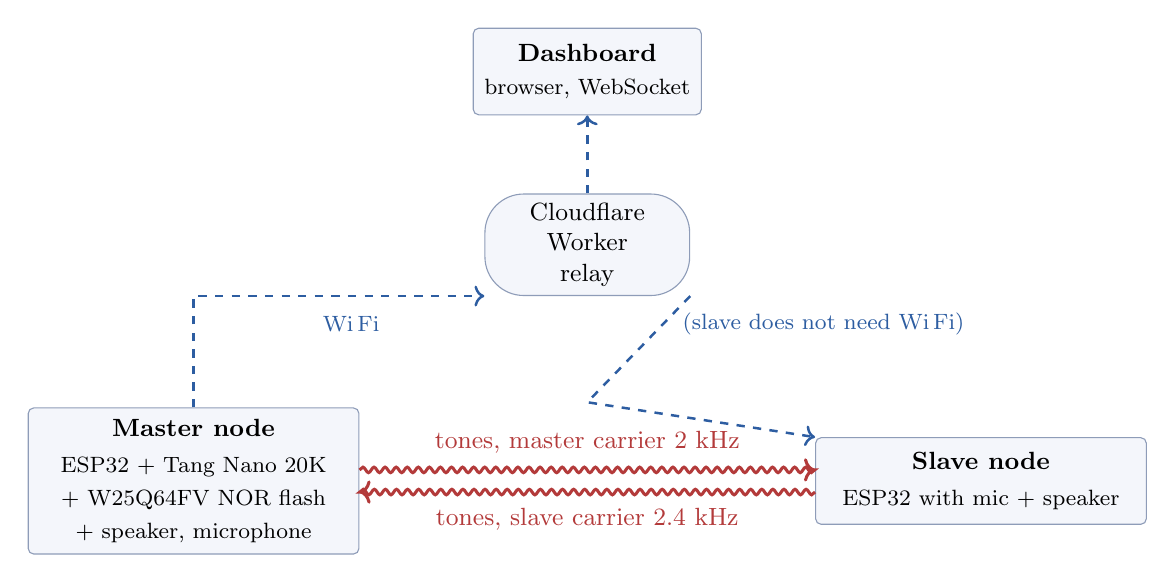
\begin{tikzpicture}[
    every node/.style={font=\small},
    box/.style={draw=boxstroke, fill=boxbg, rounded corners=2pt, minimum height=1.1cm, align=center, inner sep=4pt},
    relay/.style={draw=boxstroke, fill=boxbg, rounded corners=14pt, minimum width=2.6cm, minimum height=1.2cm, align=center},
    audio/.style={->, line width=1.1pt, accentred, decorate, decoration={snake, amplitude=1pt, segment length=4pt}},
    wifi/.style={->, line width=0.9pt, busblue, dashed},
    wire/.style={->, line width=0.7pt, gray!60!black}
]

% Master block
\node[box, minimum width=4.2cm] (master) at (0,0) {%
    \textbf{Master node}\\[2pt]
    \footnotesize ESP32 + Tang Nano 20K\\[1pt]
    \footnotesize + W25Q64FV NOR flash\\[1pt]
    \footnotesize + speaker, microphone
};

% Slave block
\node[box, minimum width=4.2cm] (slave) at (10,0) {%
    \textbf{Slave node}\\[2pt]
    \footnotesize ESP32 with mic + speaker
};

% Cloud relay
\node[relay] (cloud) at (5, 3) {Cloudflare\\ Worker\\ relay};

% Dashboard
\node[box, minimum width=2.6cm] (dash) at (5, 5.2) {%
    \textbf{Dashboard}\\[1pt]
    \footnotesize browser, WebSocket
};

% Acoustic links
\draw[audio] ([yshift=4pt]master.east) -- node[above, yshift=2pt, accentred] {tones, master carrier 2 kHz} ([yshift=4pt]slave.west);
\draw[audio] ([yshift=-4pt]slave.west) -- node[below, yshift=-2pt, accentred] {tones, slave carrier 2.4 kHz} ([yshift=-4pt]master.east);

% WiFi link
\draw[wifi] (master.north) |- (cloud.south west) coordinate (c1);
\draw[wifi] (cloud.south east) coordinate (c2) -- (5,1) -- (slave.north west);
\draw[wifi] (cloud.north) -- (dash.south);

\node[busblue, font=\footnotesize] at (2.0, 2.0) {Wi\,Fi};
\node[busblue, font=\footnotesize] at (8.0, 2.0) {(slave does not need Wi\,Fi)};

\end{tikzpicture}
\caption{System level view. The two boards talk over the air using audible
tones (squiggly red arrows). The master also has a Wi\,Fi link to a
Cloudflare Worker that relays WebSocket traffic to a browser dashboard.}
\label{fig:system}
\end{figure}

The acoustic link is the only path between master and slave. There is no
shared cable, no Bluetooth, no I2C. Whatever the two have to say to each
other (presence requests, identification, OK acknowledgements, abort) has
to be encoded into tones and demodulated on the other side. We will come
back to the protocol in Section~\ref{sec:protocol}.

The Wi\,Fi link is convenience plumbing for the dashboard, not for the
acoustic protocol. A Cloudflare Worker (running on Cloudflare's edge
network) acts as a thin WebSocket relay: the master connects to it over
TLS, the browser connects to it over TLS, the Worker shovels messages
between the two. This lets the user open the dashboard on a phone or
laptop from anywhere without needing the master to expose a public IP.

\subsection{The master, opened up}

\begin{figure}[H]
\centering
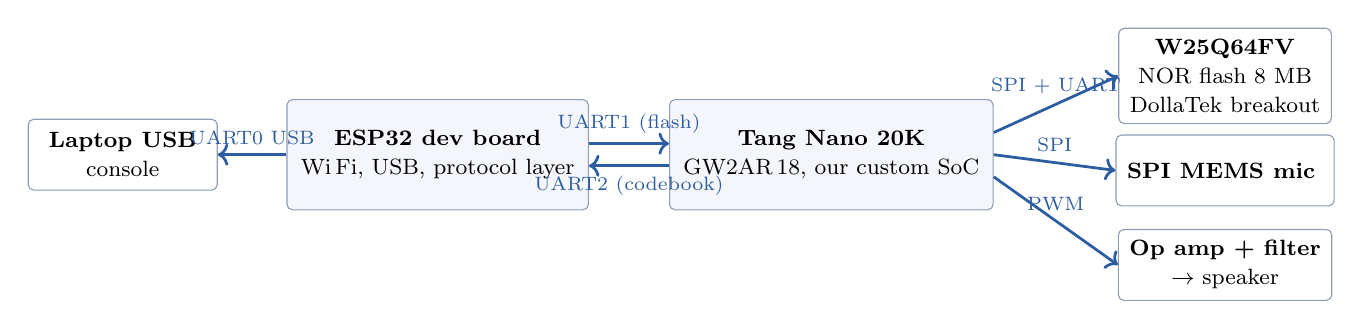
\begin{tikzpicture}[
    every node/.style={font=\footnotesize},
    chip/.style={draw=boxstroke, fill=boxbg, rounded corners=2pt, minimum height=1.4cm, align=center, inner sep=5pt},
    ext/.style={draw=boxstroke, fill=white, rounded corners=2pt, minimum height=0.9cm, align=center, inner sep=4pt},
    bus/.style={->, line width=1pt, busblue},
    pwr/.style={->, line width=0.8pt, accentred}
]

\node[chip, minimum width=3.4cm] (esp) at (0,0) {%
    \textbf{ESP32 dev board}\\[1pt]
    \footnotesize Wi\,Fi, USB, protocol layer
};

\node[chip, minimum width=3.4cm] (fpga) at (5,0) {%
    \textbf{Tang Nano 20K}\\[1pt]
    \footnotesize GW2AR\,18, our custom SoC
};

\node[ext, minimum width=2.4cm] (nor) at (10,1.0) {%
    \textbf{W25Q64FV}\\[1pt]
    \footnotesize NOR flash 8 MB\\[1pt]
    \footnotesize DollaTek breakout
};

\node[ext, minimum width=2.4cm] (mic) at (10,-0.2) {%
    \textbf{SPI MEMS mic}
};

\node[ext, minimum width=2.4cm] (spk) at (10,-1.4) {%
    \textbf{Op amp + filter}\\[1pt]
    \footnotesize $\rightarrow$ speaker
};

\node[ext, minimum width=2.4cm] (usb) at (-4,0) {%
    \textbf{Laptop USB}\\[1pt]
    \footnotesize console
};

% Connections ESP32 to FPGA
\draw[bus] ([yshift=4pt]esp.east) -- node[above, font=\scriptsize, busblue] {UART1 (flash)} ([yshift=4pt]fpga.west);
\draw[bus] ([yshift=-4pt]fpga.west) -- node[below, font=\scriptsize, busblue] {UART2 (codebook)} ([yshift=-4pt]esp.east);

% ESP32 to USB
\draw[bus] ([yshift=0pt]esp.west) -- node[above, font=\scriptsize, busblue] {UART0 USB} (usb.east);

% FPGA to externals
\draw[bus] ([yshift=8pt]fpga.east) -- node[above, font=\scriptsize, busblue] {SPI + UART} (nor.west);
\draw[bus] ([yshift=0pt]fpga.east) -- node[above, font=\scriptsize, busblue] {SPI} (mic.west);
\draw[bus] ([yshift=-8pt]fpga.east) -- node[above, font=\scriptsize, busblue] {PWM} (spk.west);

\end{tikzpicture}
\caption{Master node, opened up. The ESP32 talks to the FPGA via two
independent UART links (one for flash storage, one for the audio codebook).
The FPGA talks to the W25Q64FV NOR flash, the SPI MEMS microphone, and the
speaker output stage. The ESP32 also exposes a USB serial console for the
laptop side, used during development.}
\label{fig:master}
\end{figure}

A few design choices worth mentioning here:

\begin{itemize}
    \item The W25Q64FV NOR flash is wired \emph{directly to the FPGA}, not
          to the ESP32. The FPGA hosts the SPI master and a state machine
          (\texttt{flash\_ctrl}) that exposes a higher level UART protocol
          to the ESP32, with opcodes like ``append log record'',
          ``read settings'', ``clear log''. This was a course requirement:
          the persistent storage controller had to live on the FPGA, not
          in the application processor.
    \item The audio chain (microphone in, speaker out) lives entirely on
          the FPGA. The ESP32 only sees the \emph{decoded symbols} (the
          letters \texttt{a}, \texttt{b}, \texttt{c}, \texttt{A}, \texttt{B},
          \texttt{C}) coming out of the audio codebook UART. It never
          touches raw audio samples.
    \item The ESP32 runs the protocol layer (presence request, abort,
          retry logic), the WebSocket client toward Cloudflare, and the
          web dashboard JSON shaping. It is a thin orchestrator, not a
          DSP.
\end{itemize}

% =====================================================================
\section{The FPGA SoC, top level view}
\label{sec:soc}
% =====================================================================

The Gowin GW2AR\,18 carries our custom SoC. The chip is a 20k LUT class
FPGA with embedded 8 MB SDRAM die inside the same package (this is what
the ``\,AR\,'' suffix denotes in the part number). The SDRAM is reachable
through dedicated pins of the FPGA fabric, not through external soldering.

\subsection{High level block diagram}

\begin{figure}[H]
\centering
\resizebox{\textwidth}{!}{%
\begin{tikzpicture}[
    every node/.style={font=\small},
    block/.style={draw, fill=boxbg, line width=0.8pt, minimum width=2.9cm, minimum height=1.8cm, align=center, inner sep=4pt},
    bigblock/.style={draw, fill=boxbg, line width=0.8pt, minimum width=2.9cm, minimum height=2.8cm, align=center, inner sep=4pt},
    bus/.style={line width=2.2pt, busblue},
    busarrow/.style={-{Triangle[length=10pt, width=10pt]}, line width=2pt, busblue},
    bitap/.style={draw, fill=busblue!25, line width=0.7pt, minimum size=0.42cm, inner sep=0pt},
    bidi/.style={Stealth-Stealth, line width=0.6pt},
    pin/.style={circle, draw, fill=white, line width=0.6pt, inner sep=1pt, minimum size=5pt},
    pinlbl/.style={font=\footnotesize},
    arrlbl/.style={font=\scriptsize, midway, sloped, fill=white, inner sep=0.5pt}
]

% Main vertical bus and big arrows top + bottom
\draw[bus] (0, -16) -- (0, 16);
\draw[busarrow] (0, 16) -- (0, 17.4);
\draw[busarrow] (0, -16) -- (0, -17.4);
\node[busblue, anchor=center, font=\bfseries] at (0, 17.9) {On Chip Bus};

% =========================
% LEFT COLUMN OF BLOCKS
% =========================

% --- rPLL (top left, fed by xtal external pin) ---
\node[block, fill=accentred!10] (pll) at (-7, 14) {%
    \textbf{rPLL}\\
    \footnotesize 27 MHz $\to$ 40.5/100 MHz\\
    \footnotesize phase shifted
};
% xtal external pin
\node[pin] (xtal) at (-12, 14) {};
\node[pinlbl, anchor=east] at (xtal.west) {XTAL 27 MHz};
\draw[line width=0.7pt] (xtal) -- (pll.west);

% Clock connection from PLL to bus (no data/ctrl/addr, just clock distribution)
\draw[->, line width=1pt, accentred] (pll.east) -- (-0.2, 14);
\node[font=\footnotesize, accentred!60!black, anchor=south] at (-3.5, 14) {clk};

% --- uP Core ---
\node[block] (cpu) at (-7, 11) {%
    \textbf{uP Core}\\
    \footnotesize Gowin soft CPU\\
    \footnotesize @ 40.5 MHz
};
\draw[bidi] (cpu.east) ++(0, 0.55) -- ++(3.4, 0) node[arrlbl, above]{data};
\draw[bidi] (cpu.east) ++(0, 0.0)  -- ++(3.4, 0) node[arrlbl, above]{control};
\draw[bidi] (cpu.east) ++(0, -0.55) -- ++(3.4, 0) node[arrlbl, above]{address};
\node[bitap] (bicpu) at (-2.6, 10.4) {};
\draw[line width=0.6pt] (-3.6, 10.45) -- (bicpu.north);
\draw[->, line width=0.6pt] (bicpu.east) -- (-0.2, 10.4);

% --- SDRAM Controller (taller) ---
\node[bigblock] (sdr) at (-7, 7.5) {%
    \textbf{SDRAM}\\
    \textbf{Controller}\\[3pt]
    \footnotesize bus @ 40.5 MHz\\
    \footnotesize DRAM @ 100 MHz\\
    \footnotesize phase shift $\sim 90^\circ$
};
\draw[bidi] (sdr.east) ++(0, 0.85) -- ++(3.4, 0) node[arrlbl, above]{data};
\draw[bidi] (sdr.east) ++(0, 0.25)  -- ++(3.4, 0) node[arrlbl, above]{control};
\draw[bidi] (sdr.east) ++(0, -0.35) -- ++(3.4, 0) node[arrlbl, above]{address};
\node[bitap] (bisdr) at (-2.6, 6.6) {};
\draw[line width=0.6pt] (-3.6, 7.15) -- (bisdr.north);
\draw[->, line width=0.6pt] (bisdr.east) -- (-0.2, 6.6);

% External SDRAM pins
\foreach \y/\name in {8.7/sdram\_a[12:0], 8.2/sdram\_dq[15:0], 7.7/{ /RAS}, 7.2/{ /CAS}, 6.7/{ /WE}, 6.2/{ /CS}, 5.7/clock} {
  \node[pin] (sp\y) at (-12, \y) {};
  \node[pinlbl, anchor=east] at (sp\y.west) {\name};
  \draw[line width=0.6pt] (sp\y) -- ($(sdr.west) + (0, \y - 7.5)$);
}

% --- HW Accelerator ---
\node[block] (accel) at (-7, 4) {%
    \textbf{HW Accelerator}\\
    \footnotesize SPI $\to$ BSRAM $\to$ FFT\\
    \footnotesize $\to$ SDRAM
};
\draw[bidi] (accel.east) ++(0, 0.55) -- ++(3.4, 0) node[arrlbl, above]{data};
\draw[bidi] (accel.east) ++(0, 0.0)  -- ++(3.4, 0) node[arrlbl, above]{control};
\draw[bidi] (accel.east) ++(0, -0.55) -- ++(3.4, 0) node[arrlbl, above]{address};
\node[bitap] (biacc) at (-2.6, 3.4) {};
\draw[line width=0.6pt] (-3.6, 3.45) -- (biacc.north);
\draw[->, line width=0.6pt] (biacc.east) -- (-0.2, 3.4);

% --- Audio Decoder ---
\node[block] (dec) at (-7, 1.0) {%
    \textbf{Audio Decoder}\\
    \footnotesize tone detect\\
    \footnotesize $\pm 3$ local max
};
\draw[bidi] (dec.east) ++(0, 0.55) -- ++(3.4, 0) node[arrlbl, above]{data};
\draw[bidi] (dec.east) ++(0, 0.0)  -- ++(3.4, 0) node[arrlbl, above]{control};
\draw[bidi] (dec.east) ++(0, -0.55) -- ++(3.4, 0) node[arrlbl, above]{address};
\node[bitap] (bidec) at (-2.6, 0.4) {};
\draw[line width=0.6pt] (-3.6, 0.45) -- (bidec.north);
\draw[->, line width=0.6pt] (bidec.east) -- (-0.2, 0.4);

% --- NOR Flash Controller ---
\node[block] (flash) at (-7, -2.0) {%
    \textbf{NOR flash ctrl}\\
    \footnotesize \texttt{flash\_ctrl} FSM\\
    \footnotesize SPI div $\div 64$
};
\draw[bidi] (flash.east) ++(0, 0.55) -- ++(3.4, 0) node[arrlbl, above]{data};
\draw[bidi] (flash.east) ++(0, 0.0)  -- ++(3.4, 0) node[arrlbl, above]{control};
\draw[bidi] (flash.east) ++(0, -0.55) -- ++(3.4, 0) node[arrlbl, above]{address};
\node[bitap] (bifl) at (-2.6, -2.6) {};
\draw[line width=0.6pt] (-3.6, -2.55) -- (bifl.north);
\draw[->, line width=0.6pt] (bifl.east) -- (-0.2, -2.6);

% External flash pins
\foreach \y/\name in {-1.0/SCK, -1.5/CS, -2.0/MOSI, -2.5/MISO} {
  \node[pin] (fp\y) at (-12, \y) {};
  \node[pinlbl, anchor=east] at (fp\y.west) {flash \name};
  \draw[line width=0.6pt] (fp\y) -- ($(flash.west) + (0, \y - (-2.0))$);
}

% --- UART char flash ---
\node[block] (uart1) at (-7, -5.0) {%
    \textbf{UART char}\\
    \footnotesize flash link\\
    \footnotesize baud div $\div 352$
};
\draw[bidi] (uart1.east) ++(0, 0.55) -- ++(3.4, 0) node[arrlbl, above]{data};
\draw[bidi] (uart1.east) ++(0, 0.0)  -- ++(3.4, 0) node[arrlbl, above]{control};
\draw[bidi] (uart1.east) ++(0, -0.55) -- ++(3.4, 0) node[arrlbl, above]{address};
\node[bitap] (biu1) at (-2.6, -5.6) {};
\draw[line width=0.6pt] (-3.6, -5.55) -- (biu1.north);
\draw[->, line width=0.6pt] (biu1.east) -- (-0.2, -5.6);

\node[pin] (u1tx) at (-12, -4.6) {};
\node[pinlbl, anchor=east] at (u1tx.west) {flash UART TX};
\draw[line width=0.6pt] (u1tx) -- ($(uart1.west) + (0, 0.4)$);
\node[pin] (u1rx) at (-12, -5.4) {};
\node[pinlbl, anchor=east] at (u1rx.west) {flash UART RX};
\draw[line width=0.6pt] (u1rx) -- ($(uart1.west) + (0, -0.4)$);

% --- UART char codebook ---
\node[block] (uart2) at (-7, -8.0) {%
    \textbf{UART char}\\
    \footnotesize codebook link\\
    \footnotesize baud div $\div 352$
};
\draw[bidi] (uart2.east) ++(0, 0.55) -- ++(3.4, 0) node[arrlbl, above]{data};
\draw[bidi] (uart2.east) ++(0, 0.0)  -- ++(3.4, 0) node[arrlbl, above]{control};
\draw[bidi] (uart2.east) ++(0, -0.55) -- ++(3.4, 0) node[arrlbl, above]{address};
\node[bitap] (biu2) at (-2.6, -8.6) {};
\draw[line width=0.6pt] (-3.6, -8.55) -- (biu2.north);
\draw[->, line width=0.6pt] (biu2.east) -- (-0.2, -8.6);

\node[pin] (u2tx) at (-12, -7.6) {};
\node[pinlbl, anchor=east] at (u2tx.west) {codebook TX};
\draw[line width=0.6pt] (u2tx) -- ($(uart2.west) + (0, 0.4)$);
\node[pin] (u2rx) at (-12, -8.4) {};
\node[pinlbl, anchor=east] at (u2rx.west) {codebook RX};
\draw[line width=0.6pt] (u2rx) -- ($(uart2.west) + (0, -0.4)$);

% --- Boot ROM (bottom left) ---
\node[block] (boot) at (-7, -11) {%
    \textbf{Boot ROM}\\
    \footnotesize init code
};
\draw[bidi] (boot.east) ++(0, 0.55) -- ++(3.4, 0) node[arrlbl, above]{data};
\draw[bidi] (boot.east) ++(0, 0.0)  -- ++(3.4, 0) node[arrlbl, above]{control};
\draw[bidi] (boot.east) ++(0, -0.55) -- ++(3.4, 0) node[arrlbl, above]{address};
\node[bitap] (bibt) at (-2.6, -11.6) {};
\draw[line width=0.6pt] (-3.6, -11.55) -- (bibt.north);
\draw[->, line width=0.6pt] (bibt.east) -- (-0.2, -11.6);

% =========================
% RIGHT COLUMN OF BLOCKS
% =========================

% --- 10 bit PWM Speaker ---
\node[block] (pwms) at (7, 11) {%
    \textbf{10 bit PWM}\\
    \footnotesize speaker, DDS\\
    \footnotesize + tone counter
};
\draw[bidi] (pwms.west) ++(0, 0.55) -- ++(-3.4, 0) node[arrlbl, above]{data};
\draw[bidi] (pwms.west) ++(0, 0.0)  -- ++(-3.4, 0) node[arrlbl, above]{control};
\draw[bidi] (pwms.west) ++(0, -0.55) -- ++(-3.4, 0) node[arrlbl, above]{address};
\node[bitap] (bipwms) at (2.6, 10.4) {};
\draw[line width=0.6pt] (3.6, 10.45) -- (bipwms.north);
\draw[->, line width=0.6pt] (bipwms.west) -- (0.2, 10.4);

\node[pin] (spk) at (12, 11) {};
\node[pinlbl, anchor=west] at (spk.east) {Speaker out (PWM)};
\draw[line width=0.6pt] (pwms.east) -- (spk);

% --- 4 bit PWM LED ---
\node[block] (pwml) at (7, 8) {%
    \textbf{4 bit PWM}\\
    \footnotesize LED
};
\draw[bidi] (pwml.west) ++(0, 0.55) -- ++(-3.4, 0) node[arrlbl, above]{data};
\draw[bidi] (pwml.west) ++(0, 0.0)  -- ++(-3.4, 0) node[arrlbl, above]{control};
\draw[bidi] (pwml.west) ++(0, -0.55) -- ++(-3.4, 0) node[arrlbl, above]{address};
\node[bitap] (bipwml) at (2.6, 7.4) {};
\draw[line width=0.6pt] (3.6, 7.45) -- (bipwml.north);
\draw[->, line width=0.6pt] (bipwml.west) -- (0.2, 7.4);

\node[pin] (led) at (12, 8) {};
\node[pinlbl, anchor=west] at (led.east) {LED};
\draw[line width=0.6pt] (pwml.east) -- (led);

% --- 1 bit OUT GPIO ---
\node[block] (gpio) at (7, 5.2) {%
    \textbf{1 bit OUT}\\
    \textbf{GPIO}\\
    \footnotesize tied to '1'
};
\draw[bidi] (gpio.west) ++(0, 0.55) -- ++(-3.4, 0) node[arrlbl, above]{data};
\draw[bidi] (gpio.west) ++(0, 0.0)  -- ++(-3.4, 0) node[arrlbl, above]{control};
\draw[bidi] (gpio.west) ++(0, -0.55) -- ++(-3.4, 0) node[arrlbl, above]{address};
\node[bitap] (bigpio) at (2.6, 4.6) {};
\draw[line width=0.6pt] (3.6, 4.65) -- (bigpio.north);
\draw[->, line width=0.6pt] (bigpio.west) -- (0.2, 4.6);

\node[pin] (gpiop) at (12, 5.2) {};
\node[pinlbl, anchor=west] at (gpiop.east) {gpio\_1\_o (must be 1)};
\draw[line width=0.6pt] (gpio.east) -- (gpiop);

% --- SPI Master for mic ---
\node[block] (spi) at (7, 2.2) {%
    \textbf{SPI Master}\\
    \footnotesize for mic\\
    \footnotesize prescaler $\div 8$
};
\draw[bidi] (spi.west) ++(0, 0.55) -- ++(-3.4, 0) node[arrlbl, above]{data};
\draw[bidi] (spi.west) ++(0, 0.0)  -- ++(-3.4, 0) node[arrlbl, above]{control};
\draw[bidi] (spi.west) ++(0, -0.55) -- ++(-3.4, 0) node[arrlbl, above]{address};
\node[bitap] (bispi) at (2.6, 1.6) {};
\draw[line width=0.6pt] (3.6, 1.65) -- (bispi.north);
\draw[->, line width=0.6pt] (bispi.west) -- (0.2, 1.6);

\foreach \y/\name in {3.0/SPICLK, 2.6/MISO, 2.2/MOSI, 1.8/SPISS} {
  \node[pin] (mp\y) at (12, \y) {};
  \node[pinlbl, anchor=west] at (mp\y.east) {mic \name};
  \draw[line width=0.6pt] ($(spi.east) + (0, \y - 2.2)$) -- (mp\y);
}

% --- Timer ---
\node[block] (tmr) at (7, -1.0) {%
    \textbf{Timer}\\
    \footnotesize 32 bit counter
};
\draw[bidi] (tmr.west) ++(0, 0.55) -- ++(-3.4, 0) node[arrlbl, above]{data};
\draw[bidi] (tmr.west) ++(0, 0.0)  -- ++(-3.4, 0) node[arrlbl, above]{control};
\draw[bidi] (tmr.west) ++(0, -0.55) -- ++(-3.4, 0) node[arrlbl, above]{address};
\node[bitap] (bitm) at (2.6, -1.6) {};
\draw[line width=0.6pt] (3.6, -1.55) -- (bitm.north);
\draw[->, line width=0.6pt] (bitm.west) -- (0.2, -1.6);

% --- TX char ctrl from mem ---
\node[block] (txctl) at (7, -4) {%
    \textbf{TX char ctrl}\\
    \footnotesize from mem
};
\draw[bidi] (txctl.west) ++(0, 0.55) -- ++(-3.4, 0) node[arrlbl, above]{data};
\draw[bidi] (txctl.west) ++(0, 0.0)  -- ++(-3.4, 0) node[arrlbl, above]{control};
\draw[bidi] (txctl.west) ++(0, -0.55) -- ++(-3.4, 0) node[arrlbl, above]{address};
\node[bitap] (bitx) at (2.6, -4.6) {};
\draw[line width=0.6pt] (3.6, -4.55) -- (bitx.north);
\draw[->, line width=0.6pt] (bitx.west) -- (0.2, -4.6);

% --- UART char audio in (third UART) ---
\node[block] (uart3) at (7, -7) {%
    \textbf{UART char}\\
    \footnotesize ESP audio in
};
\draw[bidi] (uart3.west) ++(0, 0.55) -- ++(-3.4, 0) node[arrlbl, above]{data};
\draw[bidi] (uart3.west) ++(0, 0.0)  -- ++(-3.4, 0) node[arrlbl, above]{control};
\draw[bidi] (uart3.west) ++(0, -0.55) -- ++(-3.4, 0) node[arrlbl, above]{address};
\node[bitap] (biu3) at (2.6, -7.6) {};
\draw[line width=0.6pt] (3.6, -7.55) -- (biu3.north);
\draw[->, line width=0.6pt] (biu3.west) -- (0.2, -7.6);

% Power pins (left, free standing)
\node[pinlbl, anchor=east] at (-12, -10) {VDD = 3.3 V};
\draw[line width=0.6pt] (-12, -10) -- (-10, -10);
\draw[line width=0.6pt] (-10, -10) -- (-10, -10.6);
\node[pinlbl, anchor=east] at (-12, -10.8) {GND};
\draw[line width=0.6pt] (-12, -10.8) -- (-10, -10.8);
\draw[line width=0.6pt] (-10.2, -10.8) -- (-9.8, -10.8);
\draw[line width=0.6pt] (-10.1, -10.95) -- (-9.9, -10.95);
\draw[line width=0.6pt] (-10.05, -11.1) -- (-9.95, -11.1);

% SoC outer box
\begin{scope}[on background layer]
\node[draw, line width=1.2pt, fit=(pll)(cpu)(sdr)(accel)(dec)(flash)(uart1)(uart2)(boot)(pwms)(pwml)(gpio)(spi)(tmr)(txctl)(uart3), inner sep=18pt, rounded corners=4pt] (socbox) {};
\end{scope}
\node[anchor=south east, font=\bfseries\large] at (socbox.south east) {\textbf{SoC} \quad};

\end{tikzpicture}%
}
\caption{SoC top level, classic Avalon style. Every peripheral connects
to the central on chip bus through three bidirectional bus ports
(\emph{data}, \emph{control}, \emph{address}) and a bus interface tap
shown as a small blue square. The big triangular arrows at the top and
bottom of the central bus mark the bus continuation toward additional
slaves not visible in this view. External pins of the SoC are shown as
small circles on the left and right margins, with their identifier label.
The rPLL block at the top sits above the bus and distributes the clock
tree to every peripheral. Compared to the original course template the
DMA controller is no longer present: it has been replaced by the HW
Accelerator block, a streaming pipeline that piggybacks BSRAM and the
FFT engine between the SPI microphone and the SDRAM controller without
involving the CPU on the per sample data path.}
\label{fig:soc}
\end{figure}

\subsection{Bus and address map}

The on chip bus is a single master, multi slave Wishbone style fabric. The
soft CPU is the only initiator of transactions on the bus (the hardware
accelerator pipeline talks point to point with BSRAM and the FFT engine, it
does not go through the shared bus). Slaves are mapped at the addresses in
Table~\ref{tab:addrmap}.

\begin{table}[H]
\centering
\caption{Bus address map (slave base addresses, byte addressing).}
\label{tab:addrmap}
\begin{tabular}{lll}
\toprule
\textbf{Slave} & \textbf{Base} & \textbf{Window} \\
\midrule
Boot ROM                 & \texttt{0x0000\_0000} & 16 KB \\
SDRAM controller         & \texttt{0x1000\_0000} & 8 MB  \\
HW accelerator regs      & \texttt{0x4000\_0000} & 256 B \\
Audio decoder regs       & \texttt{0x4000\_1000} & 256 B \\
PWM speaker (10 bit)     & \texttt{0x5000\_0000} & 16 B  \\
PWM LED (4 bit)          & \texttt{0x5000\_1000} & 16 B  \\
1 bit OUT GPIO           & \texttt{0x5000\_2000} & 4 B   \\
SPI master (mic)         & \texttt{0x5000\_3000} & 32 B  \\
Timer                    & \texttt{0x5000\_4000} & 16 B  \\
NOR flash controller     & internal, UART driven & not bus mapped \\
\bottomrule
\end{tabular}
\end{table}

The NOR flash controller is special: it is a standalone block that lives
inside the FPGA fabric but does not present itself on the Wishbone bus.
It talks to the outside world through its own UART line to the ESP32 (see
Section~\ref{sec:flashctrl}). The decision was driven by the fact that the
CPU does not need to touch flash directly: all the application logic that
needs to log events lives on the ESP32, so a UART command channel is the
cleanest interface for that role.

\subsection{What changed from the course template}

The block diagram you may have seen in the course slides included a
generic DMA controller between the SPI mic and SDRAM, with the CPU
configuring DMA descriptors. Two reasons we did not keep that:

\begin{itemize}
    \item the DMA approach burns CPU cycles every time a descriptor has
          to be reprogrammed, which is awkward when samples flow at 48 kHz,
    \item the FFT block we instantiated needs samples in a very specific
          layout (256 sample window, aligned to the FFT input), and we
          ended up baking the gather and rearrange logic directly into a
          custom streaming accelerator that we control with a single
          start command from the CPU.
\end{itemize}

So in the as built system, the data path from the microphone all the way
into SDRAM is autonomous hardware. The CPU only kicks off bursts and waits
for a done interrupt. Per sample arithmetic never touches the CPU.

% =====================================================================
\section{Component deep dives}
% =====================================================================

This section walks through each block of Figure~\ref{fig:soc} and describes
its responsibilities, its register interface where it has one, and its
internal state machine where useful.

\subsection{The soft CPU}

The CPU is a Gowin provided soft core, configured with 8 KB of instruction
cache, no data cache, and the Wishbone style master interface enabled. It
runs at the same clock as the bus (40.5 MHz, derived from a PLL whose
reference is the 27 MHz onboard crystal of the Tang Nano 20K).

The CPU executes a small bare metal program (no operating system) that:

\begin{enumerate}
    \item initializes the SDRAM controller via its register window,
    \item arms the hardware accelerator with the FFT parameters,
    \item starts continuous sampling,
    \item spins on the audio decoder's status register, reading out the
          decoded tone whenever a new one is available, and emitting it
          on the codebook UART toward the ESP32.
\end{enumerate}

This is intentionally simple: heavy lifting is in dedicated hardware, the
CPU is a glorified state sequencer.

\subsection{Clock tree (rPLL plus per peripheral prescalers)}
\label{sec:clocks}

Before going into the individual peripherals it helps to look at how
clocks are distributed inside the SoC. The board provides a 27 MHz crystal
on a dedicated input pin of the GW2AR\,18. From there a Gowin \textbf{rPLL}
primitive generates two derived clocks used everywhere:

\begin{itemize}
    \item a 40.5 MHz \emph{bus clock} that drives the CPU, the on chip
          bus, the \texttt{flash\_ctrl} FSM, the audio decoder, the
          UART char modules, and most other peripherals,
    \item a 100 MHz \emph{SDRAM clock} with a programmable phase shift
          (we ended up at roughly 90 degrees of shift, see
          Section~\ref{sec:sdram}) that drives the SDRAM die.
\end{itemize}

The rPLL is configured at synthesis time via Gowin's IP catalog: input
27 MHz, output 0 at 40.5 MHz, output 1 at 100 MHz with phase shift, no
spread spectrum.

Most peripherals receive the 40.5 MHz clock but operate their I/O at a
slower rate. The way they do this varies block by block:

\begin{itemize}
    \item the \textbf{SPI master for the NOR flash} contains an internal
          counter that divides the bus clock by 64, giving a SPI SCK of
          $40.5\,\mathrm{MHz} / 64 \approx 633$ kHz. This is far below the
          chip's nominal 104 MHz max, intentionally chosen because of the
          signal integrity constraints described in Section~\ref{sec:si},
    \item the \textbf{SPI master for the MEMS microphone} divides by 8,
          giving about 5 MHz of SCK,
    \item the \textbf{UART char modules} divide the bus clock by 352 to
          obtain a 115200 baud bit rate (each bit lasts 8.68 \textmu s,
          which at 40.5 MHz is roughly 352 cycles),
    \item the \textbf{10 bit PWM speaker} uses a tone counter that
          loads the desired tone period from a register, plus a sigma
          delta accumulator that turns the desired duty cycle into a
          single bit PWM output. The carrier of the PWM (the rate at
          which the output toggles) is just the bus clock, so 40.5 MHz,
          giving plenty of distance from the audio band and trivial
          analog low pass filtering,
    \item the \textbf{audio decoder} runs at the FFT's natural rate
          (one bin per cycle in a streaming fashion), driven by a sample
          tick that fires every 1 / 48 kHz of bus clock, so roughly
          every 844 cycles.
\end{itemize}

Figure~\ref{fig:clocktree} zooms in on the clock tree.

\begin{figure}[H]
\centering
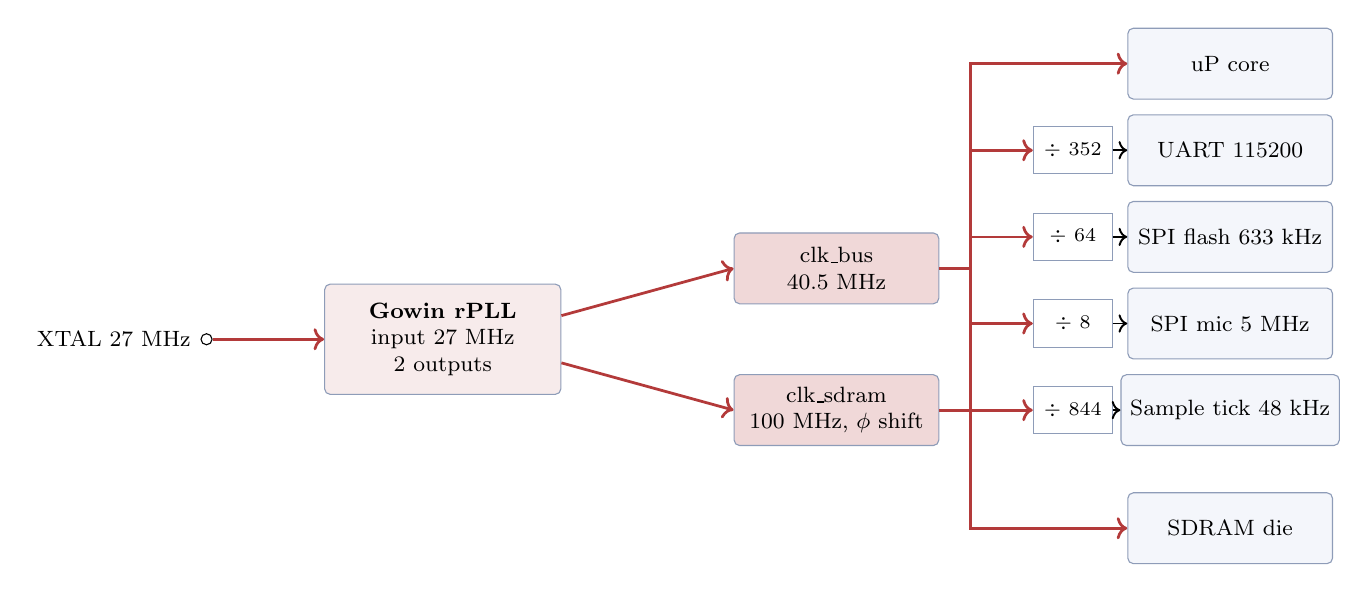
\begin{tikzpicture}[
    every node/.style={font=\footnotesize},
    blk/.style={draw=boxstroke, fill=boxbg, rounded corners=2pt, minimum width=2.6cm, minimum height=0.9cm, align=center},
    pll/.style={draw=boxstroke, fill=accentred!10, rounded corners=2pt, minimum width=3.0cm, minimum height=1.4cm, align=center},
    pin/.style={circle, draw, fill=white, inner sep=1pt, minimum size=4pt},
    clk/.style={->, line width=1.0pt, accentred},
    div/.style={draw=boxstroke, fill=white, minimum width=1.0cm, minimum height=0.6cm, align=center, font=\scriptsize}
]
% xtal
\node[pin] (xtal) at (-1.5, 0) {};
\node[anchor=east] at (xtal.west) {XTAL 27 MHz};

% PLL
\node[pll] (pll) at (1.5, 0) {\textbf{Gowin rPLL}\\ \footnotesize input 27 MHz\\ \footnotesize 2 outputs};

% Output clocks
\node[blk, fill=accentred!20] (clkbus) at (6.5, 0.9) {clk\_bus\\ 40.5 MHz};
\node[blk, fill=accentred!20] (clkdram) at (6.5, -0.9) {clk\_sdram\\ 100 MHz, $\phi$ shift};

\draw[clk] (xtal) -- (pll);
\draw[clk] (pll.east) ++(0,0.3) -- (clkbus.west);
\draw[clk] (pll.east) ++(0,-0.3) -- (clkdram.west);

% Consumers of clk_bus
\node[blk] (cpu) at (11.5, 3.5) {uP core};
\node[div] (d352a) at (9.5, 2.4) {$\div$ 352};
\node[blk] (uart) at (11.5, 2.4) {UART 115200};
\node[div] (d64) at (9.5, 1.3) {$\div$ 64};
\node[blk] (spifl) at (11.5, 1.3) {SPI flash 633 kHz};
\node[div] (d8) at (9.5, 0.2) {$\div$ 8};
\node[blk] (spimic) at (11.5, 0.2) {SPI mic 5 MHz};
\node[div] (d844) at (9.5, -0.9) {$\div$ 844};
\node[blk] (smptick) at (11.5, -0.9) {Sample tick 48 kHz};

\draw[clk] (clkbus.east) -- ++(0.4, 0) |- (cpu.west);
\draw[clk] (clkbus.east) -- ++(0.4, 0) |- (d352a.west);
\draw[clk] (clkbus.east) -- ++(0.4, 0) |- (d64.west);
\draw[clk] (clkbus.east) -- ++(0.4, 0) |- (d8.west);
\draw[clk] (clkbus.east) -- ++(0.4, 0) |- (d844.west);

\draw[->, line width=0.7pt] (d352a) -- (uart);
\draw[->, line width=0.7pt] (d64)   -- (spifl);
\draw[->, line width=0.7pt] (d8)    -- (spimic);
\draw[->, line width=0.7pt] (d844)  -- (smptick);

% Consumers of clk_sdram
\node[blk] (sdram) at (11.5, -2.4) {SDRAM die};
\draw[clk] (clkdram.east) -- ++(0.4, 0) |- (sdram.west);

\end{tikzpicture}
\caption{Clock tree. The rPLL takes the 27 MHz crystal and produces two
synchronous clocks at 40.5 MHz (bus) and 100 MHz (SDRAM, with phase shift).
Each peripheral that needs a slower clock instantiates its own integer
divider downstream of the bus clock. We did not use Gowin clock gating
primitives for any of these, simply because the divider counters are
trivial in resources and give us per peripheral control of the prescaler
ratio at synthesis time.}
\label{fig:clocktree}
\end{figure}

A practical note on the choice of divider values: every divider is a
power of 2 or a small composite number so the resulting waveform is
symmetric and the duty cycle of the derived clock is 50 percent. The
$\div 352$ for UART is the exception, because 115200 baud has no clean
ratio to 40.5 MHz: we used a fractional accumulator inside the UART
state machine to absorb the rounding error.

\subsection{SDRAM controller}
\label{sec:sdram}

The SDRAM is a 8 MB synchronous DRAM die packaged in the same module as the
GW2AR\,18 FPGA. It is reachable on dedicated pins of the FPGA. The
controller is generated from the Gowin IP catalog with the parameters
matched to the embedded die (32 Mbit \texttimes{} 16, four banks, CAS
latency 3, refresh interval 64 ms / 8192 rows).

\subsubsection{Init sequence}

After power up the SDRAM has to be put into a known state before any read
or write. Skipping any of the steps below makes the chip return garbage
forever, which is exactly what we saw the first time we tried to read back
what we had just written. The sequence we ended up running is:

\begin{enumerate}
    \item assert \texttt{CKE} (clock enable) and wait at least 200~\textmu s
          for the internal regulator to stabilize,
    \item issue a PRECHARGE ALL to bring every bank to idle,
    \item issue at least two AUTO REFRESH commands (the die requires two,
          to lock the refresh counter),
    \item program the Mode Register with CAS latency 3, burst length 1,
          sequential burst type, write burst single location,
    \item from here on, the controller is free to issue ACTIVATE / READ /
          WRITE / PRECHARGE pairs.
\end{enumerate}

\begin{figure}[H]
\centering
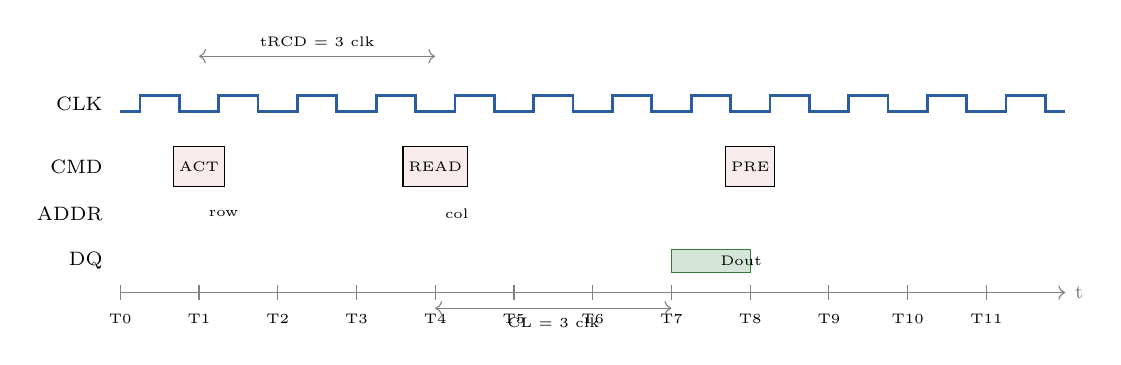
\begin{tikzpicture}[
    every node/.style={font=\scriptsize, anchor=west},
    sig/.style={line width=0.8pt},
    clk/.style={line width=1pt, busblue},
    cmd/.style={line width=1pt, accentred},
    cmdbox/.style={draw, fill=accentred!10, font=\tiny, inner sep=2pt, minimum height=0.5cm, anchor=center}
]
% Time axis
\draw[->, gray] (0,-2.4) -- (12,-2.4) node[right]{t};
\foreach \x/\lbl in {0/T0,1/T1,2/T2,3/T3,4/T4,5/T5,6/T6,7/T7,8/T8,9/T9,10/T10,11/T11} {
    \draw[gray] (\x, -2.3) -- (\x, -2.5);
    \node[anchor=north, font=\tiny] at (\x, -2.55) {\lbl};
}
% Clock
\node[anchor=east] at (-0.1, 0) {CLK};
\foreach \x in {0,1,2,3,4,5,6,7,8,9,10,11} {
    \draw[clk] (\x, -0.1) -- (\x+0.25, -0.1) -- (\x+0.25, 0.1) -- (\x+0.75, 0.1) -- (\x+0.75, -0.1) -- (\x+1, -0.1);
}
% Command labels
\node[anchor=east] at (-0.1, -0.8) {CMD};
\node[cmdbox] at (1, -0.8) {ACT};
\node[cmdbox] at (4, -0.8) {READ};
\node[cmdbox] at (8, -0.8) {PRE};
% Address
\node[anchor=east] at (-0.1, -1.4) {ADDR};
\node[font=\tiny] at (1, -1.4) {row};
\node[font=\tiny] at (4, -1.4) {col};
% Data
\node[anchor=east] at (-0.1, -2.0) {DQ};
\draw[fill=accentgreen!20, draw=accentgreen] (7, -2.15) rectangle (8, -1.85);
\node[font=\tiny] at (7.5, -2.0) {Dout};

% Annotation: tRCD
\draw[<->, gray] (1, 0.6) -- (4, 0.6);
\node[font=\tiny, anchor=south] at (2.5, 0.6) {tRCD = 3 clk};
% Annotation: CAS latency
\draw[<->, gray] (4, -2.6) -- (7, -2.6);
\node[font=\tiny, anchor=north] at (5.5, -2.6) {CL = 3 clk};
\end{tikzpicture}
\caption{SDRAM read cycle, simplified. ACTIVATE opens the row, READ
selects the column, the chip drives the data line three clocks later (CAS
latency 3). PRECHARGE closes the row.}
\label{fig:sdram-timing}
\end{figure}

\subsubsection{Problems we had}

The first version of the controller did not respect the refresh interval
strictly. Symptom: writes appeared to work, but a read after a few seconds
came back with bits flipped. Root cause: rows that had not been refreshed
long enough lose their charge. Fix: a refresh counter inside the controller
that issues an AUTO REFRESH every 7.6~\textmu s (64 ms divided by 8192
rows). After that, retention was rock solid.

The second issue was \emph{skew} on the data lines vs the clock. At the
nominal 100 MHz SDRAM clock we generate from the PLL, even a few hundreds
of picoseconds of mismatch between the clock arriving at the SDRAM die and
the data being sampled is enough to read 0xFFFE instead of 0xFFFF. We
solved it by clocking the controller off a phase shifted copy of the bus
clock: the PLL has a programmable phase output that lets us slide the SDRAM
clock by a fraction of a period until the read data window lines up. The
empirical sweet spot ended up around 90 degrees of shift.

\subsection{Hardware accelerator pipeline}

This is the heart of the audio data path.

\begin{figure}[H]
\centering
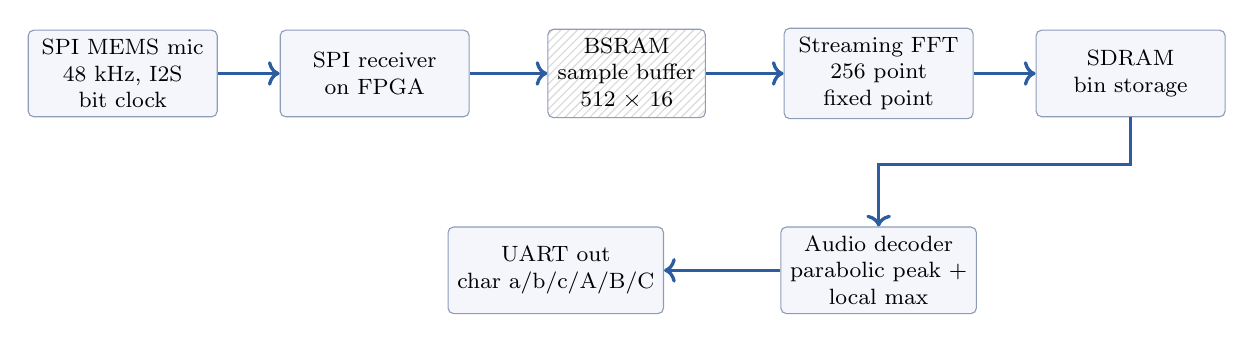
\begin{tikzpicture}[
    every node/.style={font=\footnotesize},
    blk/.style={draw=boxstroke, fill=boxbg, rounded corners=2pt, minimum width=2.4cm, minimum height=1.1cm, align=center},
    bram/.style={draw=boxstroke, fill=boxbg, rounded corners=2pt, minimum width=2.0cm, minimum height=1.1cm, align=center, pattern=north east lines, pattern color=gray!30},
    arr/.style={->, line width=1.2pt, busblue}
]
\node[blk] (mic) at (0,0) {SPI MEMS mic\\ \footnotesize 48 kHz, I2S\\ \footnotesize bit clock};
\node[blk] (spi) at (3.2,0) {SPI receiver\\ \footnotesize on FPGA};
\node[bram] (br1) at (6.4,0) {BSRAM\\ \footnotesize sample buffer\\ \footnotesize 512 \texttimes{} 16};
\node[blk] (fft) at (9.6,0) {Streaming FFT\\ \footnotesize 256 point\\ \footnotesize fixed point};
\node[blk] (sdr) at (12.8,0) {SDRAM\\ \footnotesize bin storage};

\draw[arr] (mic) -- (spi);
\draw[arr] (spi) -- (br1);
\draw[arr] (br1) -- (fft);
\draw[arr] (fft) -- (sdr);

% Audio decoder downstream
\node[blk] (dec) at (9.6, -2.5) {Audio decoder\\ \footnotesize parabolic peak +\\ \footnotesize local max};
\draw[arr] (sdr.south) -- ++(0, -0.6) -| (dec.north);

\node[blk] (uart) at (5.5, -2.5) {UART out\\ \footnotesize char a/b/c/A/B/C};
\draw[arr] (dec) -- (uart);

\end{tikzpicture}
\caption{Streaming pipeline from microphone to decoded symbol. Each stage
is autonomous: the SPI receiver pushes samples into BSRAM as they arrive,
the FFT engine pulls 256 sample windows out and produces magnitude bins
which are stored in SDRAM, the audio decoder watches the bins for tones
matching our codebook and emits a character on the UART when it sees one.}
\label{fig:audio-pipeline}
\end{figure}

\subsubsection{The FFT engine}

We use a fixed point 256 point radix 2 FFT, with input samples at 48 kHz
sample rate. The frequency bins are spaced at $48000 / 256 = 187.5$ Hz
apart. Our protocol uses these five candidate frequencies:

\begin{itemize}
    \item 2000 Hz (master carrier), bin 22 of the FFT,
    \item 2400 Hz (slave carrier),  bin 27,
    \item 2900 Hz (EOF marker),     bin 32,
    \item 3500 Hz (bit 0),          bin 39,
    \item 4500 Hz (bit 1),          bin 50.
\end{itemize}

Bins are chosen so they fall at least 5 bin distances apart, which gives
robust local maximum detection (see next subsection) and avoids spectral
leakage between adjacent tones.

\subsubsection{Audio decoder, parabolic peak interpolation}

The audio decoder looks at the five candidate bins and decides, for each
window, whether a tone is present and which one it is. Two checks per bin:

\begin{enumerate}
    \item the magnitude at the candidate bin is the local maximum across
          a $\pm 3$ neighborhood, that is the magnitude at bin $b$ is
          higher than the magnitude at bins $b-3, b-2, b-1, b+1, b+2, b+3$,
    \item the magnitude is above an amplitude threshold,
    \item a parabolic interpolation against bins $b-1, b, b+1$ confirms
          the peak is genuinely centered.
\end{enumerate}

If all three conditions hold, the decoder emits the corresponding
character. The output goes onto its own UART line back to the ESP32 where
the protocol layer turns sequences of characters into protocol patterns.

\subsubsection{The window radius problem}

A historical note that ate up a non trivial amount of debugging time. The
first version of the decoder used a $\pm 1$ neighborhood for the local
maximum check. On paper that is the most selective check, the strictest
``the peak is exactly at this bin and nowhere else''. In practice it
failed often, because the Hann window we apply before the FFT smears
energy into the neighbors, and a real tone at 2000 Hz can easily have its
peak land on bin 21 or bin 23 for a frame or two. With $\pm 1$ checking,
those frames returned ``no tone'', and the decoder missed half the symbols.

After widening the check to $\pm 3$ the false negatives disappeared. The
trade off is that two tones must be at least 7 bins apart to coexist in
the same window without confusing the decoder, but in our 5 tone codebook
the minimum spacing is 5 bins (between bit 0 at 3500 Hz and EOF at 2900
Hz, which is bin 39 minus bin 32 equals 7) so we are safe.

\subsection{PWM speaker}

The output side uses a 10 bit PWM register that drives a single FPGA pin
through an op amp buffer and an analog low pass filter (Section~\ref{sec:opamp}).
The CPU writes a target tone frequency to a register; an internal DDS
(direct digital synthesizer) generates the sine wave; the PWM compares the
DDS output to a sawtooth and emits a duty cycle modulated square wave;
the low pass smooths it back into a sine.

The tone duration is controlled by a downcounter: the CPU writes the
desired number of samples (at 27 MHz) and the speaker block runs the DDS
for exactly that many cycles, then stops. A short silence (350 ms by
default, programmable) is inserted between tones to let the receiver
finish processing the previous symbol.

\subsection{NOR flash controller (\texttt{flash\_ctrl})}
\label{sec:flashctrl}

The most complex block in the SoC by line count, and the one that gave us
the most pain on the bench. The job: take high level requests from the
ESP32 over UART (opcodes like ``append this 16 byte record'', ``save
these 32 byte settings'', ``read back this slot'', ``erase the entire
log'') and translate them into SPI transactions to the external W25Q64FV.

\subsubsection{Memory layout}

We divided the W25Q64FV's first 12 KB into three sectors of 4 KB each
(the chip's natural sector erase granularity):

\begin{itemize}
    \item Sector 0 (\texttt{0x0000}): \textbf{settings sector}, holds 32
          bytes of structured settings plus padding. Format:
          magic byte 0xA5, 15 byte device name, 2 byte auto presence
          interval, 1 byte retry count, 13 reserved bytes.
    \item Sector 1 (\texttt{0x1000}): \textbf{log A}, 256 slots of 16
          bytes each, slot \texttt{N} starts at address \texttt{0x1000 +
          N\,\texttimes\,16}.
    \item Sector 2 (\texttt{0x2000}): \textbf{log B}, same layout as log A.
\end{itemize}

Log A and log B together form a 512 slot ring buffer. Each slot is one log
record, 16 bytes, with the structure: 2 bytes sequence number, 1 byte type
character (\texttt{B} for boot, \texttt{R} for registration, \texttt{P} for
presence, \texttt{N} for note, \texttt{E} for event), 4 bytes unix
timestamp, 1 byte value, 8 bytes ASCII text.

\subsubsection{Top level state machine}

\begin{figure}[H]
\centering
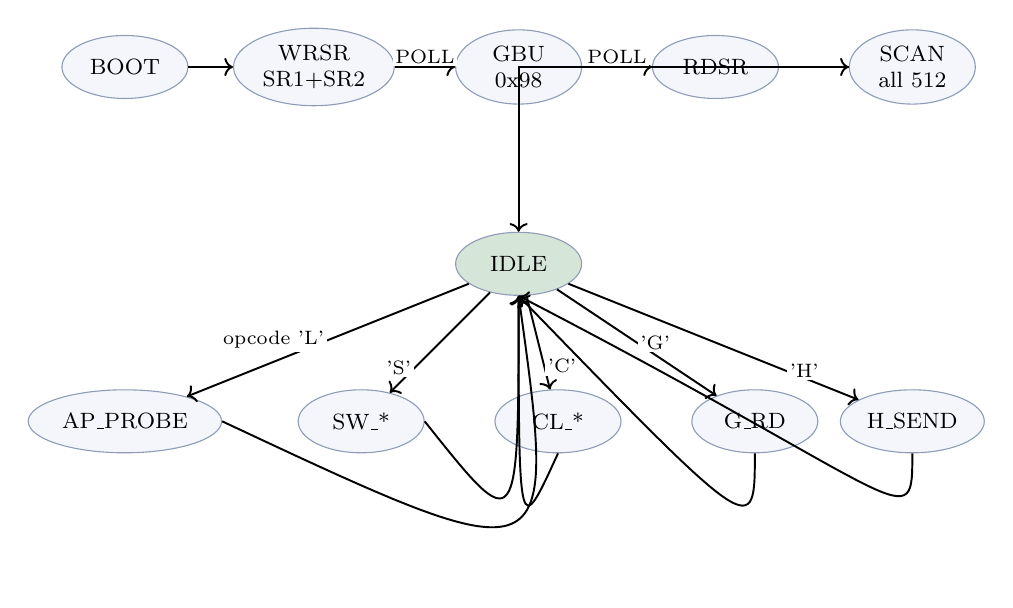
\begin{tikzpicture}[
    every node/.style={font=\footnotesize},
    state/.style={ellipse, draw=boxstroke, fill=boxbg, minimum width=1.6cm, minimum height=0.8cm, align=center, inner sep=2pt},
    arr/.style={->, line width=0.7pt},
    arrlbl/.style={font=\scriptsize, fill=white, inner sep=1pt}
]
\node[state] (boot) at (0, 0) {BOOT};
\node[state] (bwrsr) at (2.4, 0) {WRSR\\ \footnotesize SR1+SR2};
\node[state] (bgbu) at (5.0, 0) {GBU\\ \footnotesize 0x98};
\node[state] (brdsr) at (7.5, 0) {RDSR};
\node[state] (scan) at (10.0, 0) {SCAN\\ \footnotesize all 512};
\node[state, fill=accentgreen!20] (idle) at (5.0, -2.5) {IDLE};

\draw[arr] (boot) -- (bwrsr);
\draw[arr] (bwrsr) -- node[arrlbl, above] {POLL} (bgbu);
\draw[arr] (bgbu) -- node[arrlbl, above] {POLL} (brdsr);
\draw[arr] (brdsr) -- (scan);
\draw[arr] (scan) -| (idle);

% From IDLE
\node[state] (app) at (0, -4.5) {AP\_PROBE};
\node[state] (sw)  at (3.0, -4.5) {SW\_*};
\node[state] (cl)  at (5.5, -4.5) {CL\_*};
\node[state] (g)   at (8.0, -4.5) {G\_RD};
\node[state] (h)   at (10.0, -4.5) {H\_SEND};

\draw[arr] (idle) -- node[arrlbl, left] {opcode 'L'} (app);
\draw[arr] (idle) -- node[arrlbl, left, near end] {'S'} (sw);
\draw[arr] (idle) -- node[arrlbl, right, near end] {'C'} (cl);
\draw[arr] (idle) -- node[arrlbl, right] {'G'} (g);
\draw[arr] (idle) -- node[arrlbl, right, near end] {'H'} (h);

\draw[arr] (app.east) .. controls (5.5, -6.5) and (5.5, -6.5) .. (idle.south);
\draw[arr] (sw.east) .. controls (5.0, -6.0) and (5.0, -6.0) .. (idle.south);
\draw[arr] (cl.south) .. controls (5.0, -6.0) and (5.0, -6.0) .. (idle.south);
\draw[arr] (g.south) .. controls (8.0, -6.0) and (8.0, -6.0) .. (idle.south);
\draw[arr] (h.south) .. controls (10.0, -6.0) and (10.0, -5.5) .. (idle.south);

\end{tikzpicture}
\caption{High level state machine of \texttt{flash\_ctrl}. After power up
the FSM runs a boot sequence that clears block protection bits in SR1 and
SR2, runs a Global Block Unlock (opcode 0x98), reads SR1 back to confirm
the chip is unlocked, and finally scans all 512 log slots to find the head
of the ring buffer. From IDLE, opcodes drive one of the operation paths.}
\label{fig:flashctrl-fsm}
\end{figure}

The append path (opcode \texttt{L}) deserves a zoom because it is where
most of the debugging happened:

\begin{figure}[H]
\centering
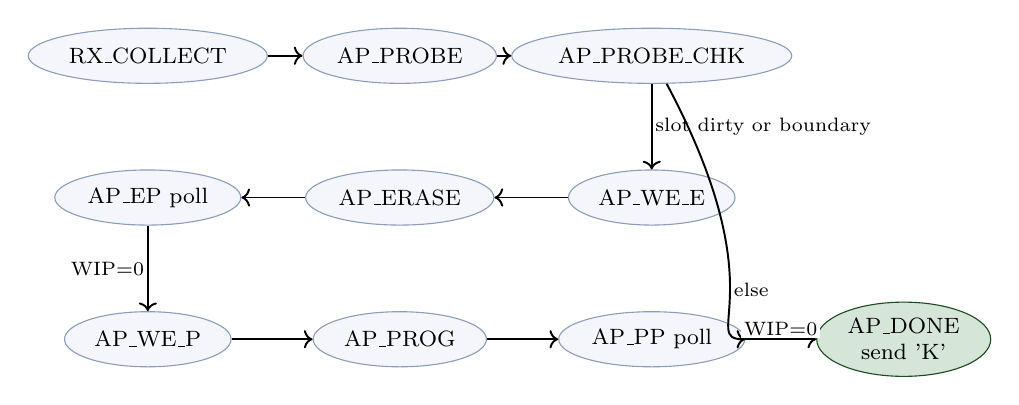
\begin{tikzpicture}[
    every node/.style={font=\footnotesize},
    state/.style={ellipse, draw=boxstroke, fill=boxbg, minimum width=1.7cm, minimum height=0.7cm, align=center, inner sep=2pt},
    accept/.style={ellipse, draw=accentgreen!60!black, fill=accentgreen!20, minimum width=1.7cm, minimum height=0.7cm, align=center, inner sep=2pt},
    arr/.style={->, line width=0.7pt},
    arrlbl/.style={font=\scriptsize, fill=white, inner sep=1pt}
]
\node[state] (rxc) at (0, 0) {RX\_COLLECT};
\node[state] (probe) at (3.2, 0) {AP\_PROBE};
\node[state] (chk) at (6.4, 0) {AP\_PROBE\_CHK};
\node[state] (wee) at (6.4, -1.8) {AP\_WE\_E};
\node[state] (era) at (3.2, -1.8) {AP\_ERASE};
\node[state] (ep)  at (0, -1.8)   {AP\_EP poll};
\node[state] (wep) at (0, -3.6)   {AP\_WE\_P};
\node[state] (prog) at (3.2, -3.6) {AP\_PROG};
\node[state] (pp)   at (6.4, -3.6) {AP\_PP poll};
\node[accept] (done) at (9.6, -3.6) {AP\_DONE\\ \footnotesize send 'K'};

\draw[arr] (rxc) -- (probe);
\draw[arr] (probe) -- (chk);
\draw[arr] (chk) -- node[arrlbl, right] {slot dirty or boundary} (wee);
\draw[arr] (chk) .. controls (8, -3) and (7.0, -3.6) .. node[arrlbl, right] {else} (pp);
\draw[arr] (wee) -- (era);
\draw[arr] (era) -- (ep);
\draw[arr] (ep) -- node[arrlbl, left] {WIP=0} (wep);
\draw[arr] (wep) -- (prog);
\draw[arr] (prog) -- (pp);
\draw[arr] (pp) -- node[arrlbl, above] {WIP=0} (done);
\end{tikzpicture}
\caption{Zoom on the log append (opcode \texttt{L}) path. After collecting
16 bytes of payload from the UART, the FSM probes the target slot's first
byte to decide whether to erase the sector first or just program directly.
This self healing behavior was added late in the project after we saw that
write parials would leave the head pointer pointing at a slot whose first
byte was not 0xFF anymore, causing later writes to AND corrupt the data.}
\label{fig:append-fsm}
\end{figure}

\subsubsection{The SCAN strategy}

At boot, the FSM has no idea where in the 512 slot ring buffer the last
valid record was written. It scans all slots and looks for valid records.

A record is considered \emph{valid} if its byte 2 (the type byte) is one
of the five allowed type characters \texttt{B}, \texttt{R}, \texttt{P},
\texttt{N}, \texttt{E}. Anything else means the slot is empty (\texttt{0xFF}
for erased) or garbage (a write that did not complete). The FSM keeps
track of the highest slot index whose record is valid, and sets the head
pointer to \texttt{(highest valid + 1) modulo 512}.

This is more robust than the obvious ``stop at the first 0xFF'' approach,
which we tried first. The naive version made the FSM stop at any hole in
the log, even if there were valid records past the hole (typical pattern
after a failed retry that left an erased slot in the middle). With the
new strategy, holes are skipped during the scan and the head ends up at
the right place.

\subsubsection{Block protection unlock at boot}

The W25Q64FV ships from the factory with block protection bits possibly
already set, depending on the supplier and the lot. Symptom of unread
protection: writes return acknowledgement but the chip silently rejects
them, leaving sectors erased forever. To bulletproof against this we do,
at every boot:

\begin{enumerate}
    \item issue \texttt{0x06 WE} (write enable),
    \item issue \texttt{0x01 WRSR} with two data bytes (\texttt{0x00},
          \texttt{0x02}): the first byte clears BP0, BP1, BP2 and SRP in
          status register 1; the second byte sets QE (Quad Enable) bit
          in status register 2, which has the side effect of disabling
          the \texttt{/HOLD\#} and \texttt{/WP\#} pin functions of the
          chip. This is critical when those pins are not pulled up on the
          board, which is exactly our case before we added the breakout
          board's pull ups,
    \item poll for the WRSR to finish,
    \item issue \texttt{0x06 WE} again,
    \item issue \texttt{0x98 Global Block Unlock}, which clears any
          individual block lock bits independent from the SR protection,
    \item poll for the operation to finish,
    \item read SR1 back and store the value into a register, expose it
          to the ESP32 via opcode \texttt{T} for diagnostic use.
\end{enumerate}

After this sequence, the chip is guaranteed to be writable for as long as
the FPGA is powered, regardless of the lot's factory state.

\subsubsection{Polling tolerance}

The page program of the W25Q64FV takes up to 3 ms; the sector erase takes
up to 400 ms. The first version of the controller used a polling counter
that timed out at 5 ms, which was enough for page program but ridiculously
short for sector erase. Symptom: every \texttt{settings\_set} returned
silently fail because the erase was still in progress when the controller
gave up and tried to start the program. Fix: raise the polling counter
ceiling to roughly 620 ms (25 million bus clocks at 40.5 MHz). At this
point the polling never times out under normal operation, and only does
when the chip is genuinely stuck.

\subsection{UART char modules}

Three instances of a small UART transmitter / receiver block live in the
SoC, one per external link. Each is parameterized by baud rate (always
115200 in our design, but the parameter exists) and exposes a one byte
wide character interface to its master logic. The blocks are register
level, no FIFOs, no interrupts: the consuming module is expected to read
the character before the next one arrives. At 115200 baud that means
roughly 87~\textmu s between characters, which is comfortable for any
state machine running at tens of MHz.

\subsection{Timer and GPIO}

The Timer block is a free running 32 bit counter driven by the bus clock,
used mainly by the bare metal program for measuring how long it took the
audio decoder to lock onto a tone (useful during development).

The 1 bit OUT GPIO has a single line that has to stay asserted at logic 1
for the whole life of the SoC. This is a Tang Nano 20K quirk: a specific
package pin must be held high for the embedded SDRAM to be active,
otherwise the SDRAM never comes out of reset. We discovered this the hard
way during the first weeks of the project (every read returned 0x0000)
and the workaround is a constant ``1'' wired to that pin via a 1 bit GPIO
register. We left a comment in the source code and a memory note: \emph{do
not, under any circumstance, set \texttt{gpio\_1\_o} to 0}.

% =====================================================================
\section{Outside the FPGA}
% =====================================================================

\subsection{The W25Q64FV NOR flash chip}

The chip is an 8 MB serial NOR flash by Winbond, in a SOIC 8 package, sat
on top of a DollaTek breakout board that exposes only 6 of the 8 pins to
the header (the missing ones, \texttt{/WP\#} and \texttt{/HOLD\#}, are
tied to VCC on the breakout PCB through pull up resistors visible as the
small SMD parts marked ``1002'' or ``182'').

\begin{figure}[H]
\centering
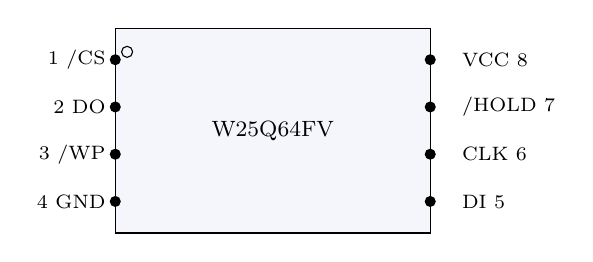
\begin{tikzpicture}[
    every node/.style={font=\footnotesize},
    chip/.style={draw, fill=boxbg, minimum width=4cm, minimum height=2.6cm},
    pin/.style={circle, fill=black, inner sep=0.6pt, minimum size=4pt},
    pinlbl/.style={font=\scriptsize}
]
\node[chip] (c) at (0,0) {W25Q64FV};
% Left pins
\node[pin] (p1) at (-2, 0.9) {}; \node[pinlbl, anchor=east] at (p1) {1 /CS\quad};
\node[pin] (p2) at (-2, 0.3) {}; \node[pinlbl, anchor=east] at (p2) {2 DO\quad};
\node[pin] (p3) at (-2, -0.3){}; \node[pinlbl, anchor=east] at (p3) {3 /WP\quad};
\node[pin] (p4) at (-2, -0.9){}; \node[pinlbl, anchor=east] at (p4) {4 GND\quad};
% Right pins
\node[pin] (p8) at (2, 0.9) {}; \node[pinlbl, anchor=west] at (p8) {\quad VCC 8};
\node[pin] (p7) at (2, 0.3) {}; \node[pinlbl, anchor=west] at (p7) {\quad /HOLD 7};
\node[pin] (p6) at (2, -0.3){}; \node[pinlbl, anchor=west] at (p6) {\quad CLK 6};
\node[pin] (p5) at (2, -0.9){}; \node[pinlbl, anchor=west] at (p5) {\quad DI 5};
% Mark pin 1
\draw (-1.85, 1.0) circle (2pt);
\end{tikzpicture}
\caption{W25Q64FV pinout, SOIC 8 package (top view). Pin 1 is the \texttt{/CS}
chip select. The DollaTek breakout exposes pins 1, 2, 5, 6 on its header,
plus VCC and GND, and ties pins 3 and 7 internally to VCC.}
\label{fig:w25q-pinout}
\end{figure}

\subsubsection{Why erase costs so much more than program}

A NOR flash cell is a floating gate transistor. Programming a single 16
byte slot is light and fast (under 3 ms, roughly 25 mA from VCC).
Erasing a 4 KB sector is heavy and slow: the chip activates an internal
charge pump that draws around 80 mA peaks for 30 ms typical (up to 400
ms worst case) to flush the floating gates of every cell in the sector
in parallel. This 3x asymmetry in current draw, combined with the 10x
to 100x longer duration, is the entire reason why we had to add a second
decoupling capacitor (see Section~\ref{sec:si}).

\subsubsection{Wiring}

\begin{table}[H]
\centering
\caption{Wiring between Tang Nano 20K FPGA, W25Q64FV breakout, and ESP32.}
\begin{tabular}{lllll}
\toprule
\textbf{Signal} & \textbf{FPGA pin} & \textbf{Bank, Vio} & \textbf{Breakout} & \textbf{ESP32 GPIO} \\
\midrule
SPI CLK   & 42 & B6, 3.3 V & CLK & ---  \\
SPI CS    & 41 & B6, 3.3 V & CS  & ---  \\
SPI MOSI  & 51 & B6, 3.3 V & DI  & ---  \\
SPI MISO  & 48 & B6, 3.3 V & DO  & ---  \\
flash UART TX & 72 & B6, 3.3 V & --- & 32 (Serial1 RX) \\
flash UART RX & 20 & B6, 3.3 V & --- & 33 (Serial1 TX) \\
3V3 / GND     & 3V3/GND     & --- & VCC / GND & --- \\
decoupling caps & --- & --- & 1 \textmu F + 10 \textmu F between VCC, GND & --- \\
\bottomrule
\end{tabular}
\end{table}

All of this is 3.3 V single ended. Common ground between Tang Nano, ESP32
and breakout is mandatory: any of the three left floating in ground breaks
the link.

\subsection{Embedded SDRAM die}

The SDRAM die is internal to the GW2AR\,18 package and not visible from
the outside, but it follows the JEDEC SDR SDRAM protocol just like a
discrete chip would. Internal organization: 4 banks, 8192 rows, 512
columns, 16 bit data bus. The pin map at the FPGA side (Table~\ref{tab:sdram-pins})
is fixed by the silicon and not user routable.

\begin{table}[H]
\centering
\caption{SDRAM pin map (internal, fixed by the GW2AR\,18 silicon).}
\label{tab:sdram-pins}
\begin{tabular}{ll}
\toprule
\textbf{Signal} & \textbf{Notes} \\
\midrule
SDRAM\_DQ[15:0] & bidirectional data \\
SDRAM\_A[12:0]  & row / column address \\
SDRAM\_BA[1:0]  & bank select \\
SDRAM\_DQM[1:0] & byte mask \\
SDRAM\_CKE      & clock enable, asserted at boot \\
SDRAM\_/CS, /RAS, /CAS, /WE & command bits \\
SDRAM\_CLK      & PLL output, phase shifted for SI \\
\bottomrule
\end{tabular}
\end{table}

\subsection{SPI MEMS microphone}

A standard SPI MEMS microphone breakout (single supply 3.3 V, output 16
bit signed PCM at 48 kHz). Wired with a tiny SCK + DOUT pair to the FPGA.
The SPI mic does not require any configuration other than asserting its
chip select.

\subsection{Op amp speaker buffer}
\label{sec:opamp}

\begin{figure}[H]
\centering
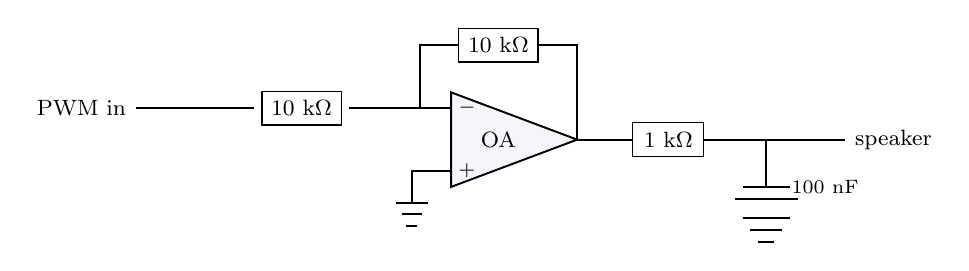
\begin{tikzpicture}[
    every node/.style={font=\footnotesize},
    res/.style={draw, fill=white, rectangle, minimum width=0.9cm, minimum height=0.3cm},
    cap/.style={},
    gnd/.style={},
    wire/.style={line width=0.7pt}
]
% Op amp triangle
\draw[wire, fill=boxbg] (4,0) -- (5.6, -0.6) -- (4, -1.2) -- cycle;
\node at (4.6, -0.6) {OA};
\node[font=\scriptsize] at (4.2, -0.2) {$-$};
\node[font=\scriptsize] at (4.2, -1.0) {$+$};

% PWM in to inverting input
\draw[wire] (0,-0.2) node[anchor=east]{PWM in} -- (1.5, -0.2);
\node[res] at (2.1, -0.2) {10 k$\Omega$};
\draw[wire] (2.7, -0.2) -- (4, -0.2);

% Feedback
\draw[wire] (3.6, -0.2) -- (3.6, 0.6) -- (5.6, 0.6) -- (5.6, -0.6);
\node[res] at (4.6, 0.6) {10 k$\Omega$};

% Op amp output to RC filter
\draw[wire] (5.6, -0.6) -- (6.3, -0.6) coordinate (out);
\node[res, anchor=west] at (6.3, -0.6) {1 k$\Omega$};
\draw[wire] (7.2, -0.6) -- (8.0, -0.6) coordinate (cnode);

% Capacitor to ground
\draw[wire] (cnode) -- (cnode |- 0,-1.2);
\draw[wire] (cnode |- 0,-1.2) ++(-0.3, 0) -- ++(0.6, 0);
\draw[wire] (cnode |- 0,-1.35) ++(-0.4, 0) -- ++(0.8, 0);
\node[anchor=west, font=\scriptsize] at (8.2, -1.2) {100 nF};
% Ground triangle
\draw[wire] (cnode |- 0,-1.6) ++(-0.3, 0) -- ++(0.6, 0);
\draw[wire] (cnode |- 0,-1.75) ++(-0.2, 0) -- ++(0.4, 0);
\draw[wire] (cnode |- 0,-1.9) ++(-0.1, 0) -- ++(0.2, 0);

% Speaker
\draw[wire] (cnode) -- (9.0, -0.6) node[anchor=west]{speaker};

% Non inverting to ground
\draw[wire] (4, -1.0) -- (3.5, -1.0) -- (3.5, -1.4);
\draw[wire] (3.5, -1.4) ++(-0.2, 0) -- ++(0.4, 0);
\draw[wire] (3.5, -1.55) ++(-0.13, 0) -- ++(0.26, 0);
\draw[wire] (3.5, -1.7) ++(-0.07, 0) -- ++(0.14, 0);
\end{tikzpicture}
\caption{Speaker output stage. The PWM signal from the FPGA is buffered
by a unity inverting op amp (configured with equal resistors so gain is
$-1$, polarity is then absorbed into the PWM table), then low pass
filtered by an RC stage tuned to roll off above the audible band, then
fed to the small 8 ohm speaker.}
\label{fig:opamp}
\end{figure}

The RC cutoff at $f = 1 / (2\pi R C) = 1 / (2 \pi \cdot 1000 \cdot 100 \cdot
10^{-9}) \approx 1.6$ kHz might look too low for our 4.5 kHz top tone, but
since the PWM carrier is at 27 MHz the goal is to kill anything above the
sound band, not to be sharp at the top of it: a softer roll off above 1.6
kHz is acceptable because the op amp + speaker combination already attenuates
the upper octaves and the receiver does not need very flat amplitude
response, only a usable peak at each tone.

\subsection{ESP32 connections}

The ESP32 dev board is wired to the FPGA on two independent UART links and
shares the same 3.3 V rail.

\begin{table}[H]
\centering
\caption{ESP32 pin assignments.}
\begin{tabular}{lll}
\toprule
\textbf{Signal} & \textbf{ESP32 GPIO} & \textbf{Notes} \\
\midrule
Serial0 (USB console) & 1 TX, 3 RX & to laptop via onboard USB to UART chip \\
Serial1 (flash link) RX & 32 & from FPGA TX pin 72 \\
Serial1 (flash link) TX & 33 & to FPGA RX pin 20 \\
Serial2 (codebook) RX   & 27 & from FPGA TX pin (audio decoder output) \\
Serial2 (codebook) TX   & 14 & to FPGA RX pin (audio codebook input) \\
\bottomrule
\end{tabular}
\end{table}

% =====================================================================
\section{Signal integrity, voltage droops, decoupling}
\label{sec:si}
% =====================================================================

This chapter could be subtitled ``what we learned about analog after
thinking we were doing digital''. None of these issues showed up in
simulation, all of them showed up on the bench, and the fixes were a mix
of hardware (a few solder joints) and firmware (slowing things down,
re-engineering polling and retry behavior).

\subsection{The W25Q64FV brownout during sector erase}

When the controller tells the W25Q64FV to erase a 4 KB sector, the chip
activates its internal charge pump to generate the high voltage required
to tunnel electrons off the floating gates. The pump draws roughly 80 mA
peaks for 30 ms (typical) up to 400 ms (worst case). The 3.3 V rail
reaching the chip arrives from the Tang Nano 20K through about 10 cm of
Dupont jumper wire, with no decoupling on the breakout other than what the
DollaTek board ships with (essentially nothing of significance).

The first version of the system had nothing at all on the VCC of the
breakout. Sector erase produced a voltage droop estimated by
$\Delta V = I \cdot t / C$ where $C$ was just the parasitic capacitance of
the wire, in the tens of pF. With a few tens of pF and 80 mA, the entire
3.3 V rail collapsed almost instantly to a fraction of a volt during the
first millisecond of the erase. The chip went into brown out, the WEL bit
got lost, the page program scheduled to run after the erase was rejected
silently, the FSM reported success, and the slot stayed empty. The user
saw ``flash\_set\_settings returned OK'' but the dashboard kept showing the
old values.

\subsection{First capacitor: 1 \textmu F}

We added a 1 \textmu F ceramic capacitor between VCC and GND of the
breakout, as close to the chip as we could solder. Recompute $\Delta V$:

\[
\Delta V = \frac{I \cdot t}{C} = \frac{0.080 \cdot 0.030}{1 \cdot 10^{-6}} = 2.4 \mathrm{V}.
\]

VCC drops by 2.4 V during a 30 ms erase, from 3.3 V down to 0.9 V. Still
well below the 2.7 V minimum spec of the chip, but better than the no cap
case. Empirical effect: the W25Q now responded to operations, page
programs of log records started working most of the time, but settings
saves still failed at high rate because the settings write does sector
erase plus page program, the cap drained during the erase and never had
time to recharge before the page program command.

\subsection{Second capacitor: 10 \textmu F in parallel}

We added a second cap in parallel, 10 \textmu F. Total: 11 \textmu F. New
droop on the same 30 ms erase:

\[
\Delta V = \frac{0.080 \cdot 0.030}{11 \cdot 10^{-6}} \approx 0.22 \mathrm{V}.
\]

VCC drops to 3.08 V during erase, comfortably above the 2.7 V minimum. The
brown out is gone, the chip behaves cleanly, settings saves return OK at
first attempt almost always.

The use of two caps of different orders of magnitude is the standard
``HF cap plus bulk cap'' configuration for decoupling: the smaller cap
(1 \textmu F, low ESR, low ESL) handles fast transients like the SPI
clock edges; the larger cap (10 \textmu F, higher ESR but much more
charge stored) handles the slow charge pump current drain during erase
and program.

\subsection{SPI clock speed reduction}

Independently from the decoupling, we found that running the SPI clock at
the 5 MHz we initially picked was too fast for the wiring. The signal
integrity of MOSI and CLK over 10 cm of Dupont wires with only one ground
return wire interleaved is bad enough that bits get sampled wrong, and we
saw partial page programs where 16 byte records came out as 2 byte truncated
text (the byte 10 and onwards came through as 0xFF instead of the intended
content). We dropped the SPI clock progressively:

\begin{itemize}
    \item 5 MHz: bad, page programs corrupt half the time,
    \item 2.5 MHz: better, still some partial corruption,
    \item 1.27 MHz: most writes succeed at first attempt,
    \item 0.633 MHz: writes succeed at first attempt almost always.
\end{itemize}

At 633 kHz a single bit lasts 1.58 \textmu s, which means every bit is
massively over the chip's setup and hold spec, with enough margin that
even the ringing on a long Dupont wire settles before the chip samples.

\subsection{Retry plus verify on the ESP32 side}

Even after the cap and the clock reduction, occasional retries are still
needed (something like 1 in 100 page programs on settings, much rarer on
log writes). The ESP32 firmware does up to 5 attempts per save: send the
data, wait for the FSM acknowledgement, read back what was written, check
that the readback matches the intended bytes byte by byte, retry if not.
After 5 attempts the firmware gives up and reports an error to the user.

Each failed retry burns one slot of the log ring buffer (because the FSM
increments the head pointer regardless), but the new SCAN strategy at boot
ignores those garbage slots because their type byte does not match the
allowed set. So no permanent harm.

\subsection{The fallback FFL diagnostics}

We added several diagnostics on the USB serial monitor so that if the
chip starts misbehaving we have a chance to debug it:

\begin{itemize}
    \item the boot prints \texttt{[flash] JEDEC = EF 40 17} to confirm
          the SPI link is alive,
    \item the boot prints \texttt{[flash] post-boot SR = 0xNN} with bit
          decoding so we see if BP or SRP are set,
    \item every page program prints \texttt{[flash] head=N (write OK
          att.X/5 ...)} or \texttt{att.X/5: VERIFY FAIL ...} so we know at
          which attempt the write succeeded,
    \item a diag dump at boot prints the first 10 slots of the log to
          confirm the SCAN found something reasonable.
\end{itemize}

% =====================================================================
\section{ESP32 firmware}
% =====================================================================

\subsection{Architecture}

The ESP32 firmware is structured as a collection of small modules with
clear ownership:

\begin{itemize}
    \item \texttt{uart\_reg}: register level driver for the ESP32 UART1
          and UART2 peripherals, no Arduino HardwareSerial dependency,
    \item \texttt{flash\_link}: high level operations against the
          \texttt{flash\_ctrl} FSM running on the FPGA, with retry and
          verify, plus a 60 record RAM cache for the display layer,
    \item \texttt{fpga\_uart\_link}: codebook layer over UART2,
          translating decoded characters into protocol patterns and
          driving the speaker through the FPGA's audio chain,
    \item \texttt{protocol}: the acoustic protocol state machine
          (presence request, retries, abort, registration),
    \item \texttt{web\_link}: WebSocket client, JSON serialization, and
          dashboard commands.
\end{itemize}

\subsection{Register level UART, instead of HardwareSerial}

Originally the firmware used \texttt{Serial1} and \texttt{Serial2} from
Arduino-ESP32, which are instances of \texttt{HardwareSerial}, which in
turn invokes the ESP IDF UART driver, which uses FreeRTOS tasks and
software ring buffers and interrupts. For the project we were asked to
demonstrate register level access, so we wrote \texttt{uart\_reg}: a small
module that talks directly to the UART peripheral registers (the FIFO
register, the CLKDIV register, the CONF0 register, the STATUS register)
of UART1 and UART2.

The headline routines:

\begin{lstlisting}[language=C++, caption={register level UART, key routines}]
void uart_reg_init(int n, int rx_pin, int tx_pin, uint32_t baud);
int  uart_reg_available(int n);                      /* RX FIFO count */
int  uart_reg_read(int n);                           /* -1 if empty */
int  uart_reg_read_bytes(int n, uint8_t *buf, int sz, uint32_t to_us);
void uart_reg_write_byte(int n, uint8_t b);
void uart_reg_write(int n, const uint8_t *buf, int sz);
void uart_reg_flush_rx(int n);

void     hw_timer_init(void);     /* TIMG0 Timer 0, free running 1 MHz */
uint64_t hw_timer_us(void);
\end{lstlisting}

The clock divider for 115200 baud at the 80 MHz APB clock is computed as:

\[
\mathrm{integer} = \left\lfloor \frac{80\,000\,000}{115200} \right\rfloor = 694, \quad
\mathrm{fractional} = \left\lfloor \frac{80\,000\,000 \cdot 16}{115200} \right\rfloor \bmod 16 = 7,
\]

with the final CLKDIV register value being $694 \;|\; (7 \ll 20) =
\texttt{0x7002B6}$. This gives an effective baud of $80\,000\,000 \div
(694 + 7/16) = 115208$ Hz, an error of 0.007 percent, within UART
tolerance.

The TIMG0 Timer 0 is configured as a free running 64 bit counter
incrementing at 1 MHz (the APB clock divided by 80) and is read by
latching the count into the LO and HI registers via the UPDATE bit. This
gives us 1 \textmu s resolution timeouts inside the UART driver without
having to touch \texttt{micros()}.

\subsection{flash\_link with retry and verify}

The data flow when the dashboard sends a \texttt{flash\_note} command:

\begin{enumerate}
    \item \texttt{web\_link} receives a JSON command on its WebSocket
          and parses it,
    \item it calls \texttt{flash\_log\_append(LOG\_NOTE, t, 0, "text")},
    \item \texttt{flash\_log\_append} composes a 16 byte record, sends
          opcode \texttt{'L'} plus the 16 bytes to the FPGA over UART1,
          waits for \texttt{'K'} acknowledgement,
    \item it then sends opcode \texttt{'H'} to read back the current
          head pointer, then \texttt{'G'} plus the slot index to read the
          16 bytes that were just written,
    \item it compares all 16 bytes against the intended record,
    \item if they match, write succeeded and the function returns true;
          if not, it retries the whole append, up to 5 attempts,
    \item regardless of outcome, the record is also pushed into a 60
          entry RAM cache so that subsequent \texttt{flash\_load}
          requests from the dashboard see it even if NOR is misbehaving.
\end{enumerate}

\texttt{flash\_set\_settings} has the same retry plus verify structure,
with the difference that it writes the 32 byte settings sector and reads
it back via opcode \texttt{'Q'} for verification.

\subsection{Defensive read of settings}

\texttt{flash\_get\_settings} is the read counterpart. After reading the
32 bytes back from the FPGA, it sanity checks before returning the data:

\begin{itemize}
    \item the magic byte at offset 0 must be \texttt{0xA5},
    \item the retry count must be between 1 and 30 (zero or 255 indicate
          a write that did not finish),
    \item the name characters must all be printable ASCII or null
          terminator.
\end{itemize}

If any of those fail, the function falls back to safe defaults
(\texttt{"Master EFES"}, 6 retries, 0 second auto presence). This way
the dashboard never displays garbled names like \texttt{"Master ?????"}
or absurd retry counts even when the underlying NOR has a partial write.

% =====================================================================
\section{The acoustic protocol}
\label{sec:protocol}
% =====================================================================

\subsection{Codebook}

The protocol uses an alternating bit codebook. Each pattern is a sequence
of two or three symbols sent on the air, with the constraint that any two
consecutive symbols must differ. This gives us robust receive detection
because the decoder triggers on \emph{change} of tone, not on absolute
silence, which is much harder to detect over a noisy channel.

The five symbols and their meanings:

\begin{table}[H]
\centering
\caption{Codebook symbols.}
\begin{tabular}{llll}
\toprule
\textbf{Symbol} & \textbf{Carrier} & \textbf{Bit} & \textbf{Notes} \\
\midrule
\texttt{a} (lowercase) & 2 kHz master  & 0 & sent by the master \\
\texttt{b}             & 2 kHz master  & 1 & sent by the master \\
\texttt{c}             & 2 kHz master  & EOF & end of frame from master \\
\texttt{A} (uppercase) & 2.4 kHz slave & 0 & sent by the slave \\
\texttt{B}             & 2.4 kHz slave & 1 & sent by the slave \\
\texttt{C}             & 2.4 kHz slave & EOF & end of frame from slave \\
\bottomrule
\end{tabular}
\end{table}

Patterns are short, two or three symbols. Examples (master to slave):

\begin{itemize}
    \item \texttt{ab} = REQ\_PRESENCE (bit 0, bit 1) length 2,
    \item \texttt{ba} = SET (assign id),
    \item \texttt{aba} = ABORT, length 3.
\end{itemize}

Patterns from slave to master use the uppercase letters, same logic.

\subsection{CSMA on the air}

Half duplex: only one party transmits at a time. The master implements a
carrier sense scheme by looking at the audio decoder output for any slave
symbol (uppercase letters) and waiting for the channel to be quiet for at
least 1 second before sending. This is done by tracking
\texttt{last\_rx\_ms} timestamps in \texttt{fpga\_uart\_link} and gating
each character before pushing to the speaker output.

\subsection{Retries}

The protocol layer on the ESP32 implements retries: a presence request
that does not see a response in 5 seconds is repeated, up to a configurable
maximum number of attempts (\texttt{tries}, persisted in the settings
sector of the NOR flash). After the maximum is reached the master gives
up and notifies the dashboard.

% =====================================================================
\section{What worked, what did not}
% =====================================================================

\subsection{Things that worked end to end}

\begin{itemize}
    \item the SoC bus and address map (no contention, no missed reads),
    \item the SDRAM controller, after the refresh interval and the
          clock phase shift were dialed in,
    \item the FFT plus parabolic peak audio decoder, the $\pm 3$ local
          maximum check made symbol detection robust,
    \item the per direction alternating bit codebook, especially after
          per direction sub codebooks were introduced for REQ\_PRESENCE
          which is the most repeated message in the system,
    \item the W25Q64FV NOR flash controller, after the long debugging
          campaign documented in Section~\ref{sec:si},
    \item the WebSocket dashboard via Cloudflare Worker,
    \item the register level UART driver on the ESP32 side, with the
          TIMG0 microsecond counter.
\end{itemize}

\subsection{Things we tried and discarded}

\begin{itemize}
    \item early on we used a generic DMA controller between the SPI mic
          and the SDRAM, with the CPU configuring descriptors. We removed
          it in favor of the streaming hardware accelerator because the
          CPU was spending too many cycles reprogramming the DMA at every
          window,
    \item we tried a tighter $\pm 1$ neighborhood for the audio decoder
          local maximum check. It made symbol detection too brittle, the
          $\pm 3$ check restored reliability,
    \item we tried using only Arduino \texttt{HardwareSerial} on the
          ESP32. It worked but did not satisfy the course requirement of
          showing register level competence, so we replaced it with
          \texttt{uart\_reg},
    \item we considered using the ESP32 internal flash via NVS for log
          storage. That would have been more reliable than the external
          NOR over Dupont wires, but the course requirement was explicit
          that the storage had to be on the FPGA side. We kept the
          W25Q64FV path.
\end{itemize}

\subsection{What still wobbles}

\begin{itemize}
    \item the wiring between Tang Nano and the W25Q breakout is still
          Dupont jumpers, which means SPI clock could not realistically
          go above 633 kHz. On a proper PCB with ground plane and short
          tracks we could probably run at 20 MHz with no retries needed,
    \item the decoupling on the breakout is 1 \textmu F plus 10 \textmu F,
          which works but is not the canonical 100 nF plus 10 \textmu F
          combo recommended by Winbond. We did not have a 100 nF ceramic
          on hand,
    \item the first SR read after power up sometimes returns 0xFF
          (chip not yet ready). The ESP32 sees this and prints a false
          ``CHIP LOCKED'' warning. Subsequent SR reads return 0x00
          correctly. We chose to leave the warning in place as it costs
          nothing and a future user might find it useful when debugging
          a truly locked chip.
\end{itemize}

\subsection{Numbers from the bench}

\begin{table}[H]
\centering
\caption{Empirical reliability of the NOR flash operations, after the
final fix set (633 kHz SPI, 11 \textmu F decoupling, retry plus verify).}
\begin{tabular}{lll}
\toprule
\textbf{Operation} & \textbf{First attempt success} & \textbf{After 5 retries} \\
\midrule
log record write (16 B) & roughly 95 percent & essentially 100 percent \\
settings save (32 B with sector erase) & roughly 85 percent & essentially 100 percent \\
read back of a record  & 100 percent & 100 percent \\
JEDEC ID read at boot  & 100 percent & 100 percent \\
\bottomrule
\end{tabular}
\end{table}

% =====================================================================
\section{Conclusions}
% =====================================================================

The EFES master node, as it stands today, is a working integration of:

\begin{itemize}
    \item a custom SoC on a Gowin GW2AR\,18 FPGA, with a streaming audio
          pipeline from SPI microphone through FFT and a tone codebook
          decoder,
    \item a NOR flash storage controller built as a finite state machine
          on the FPGA, talking SPI to a W25Q64FV chip on a Dupont breakout,
    \item an ESP32 firmware that orchestrates the higher level protocol,
          drives the dashboard over WebSocket, and accesses both the FPGA
          UART links at register level,
    \item a small, opinionated web dashboard hosted as static files and
          served through a Cloudflare Worker.
\end{itemize}

\noindent
The single most valuable lesson from the project is that for analog
mixed signal subsystems the documentation in the chip's datasheet is the
beginning of the problem, not the end. Calculations like
$\Delta V = I \cdot t / C$ should be the first thing you reach for when a
write inexplicably fails, not the last.

\appendix

% =====================================================================
\section{Quick reference card}
% =====================================================================

\begin{table}[H]
\centering
\caption{Quick reference of magic numbers used throughout the project.}
\begin{tabular}{ll}
\toprule
FPGA bus clock & 40.5 MHz \\
SDRAM clock & 100 MHz, phase shifted by roughly 90 degrees \\
Audio sample rate & 48 kHz \\
FFT size & 256 samples \\
FFT bin width & 187.5 Hz \\
NOR SPI clock & 633 kHz (SPI\_DIV = 64) \\
UART baud & 115200 \\
W25Q64FV JEDEC ID & EF 40 17 \\
Sector erase time & 30 ms typical, 400 ms max \\
Page program time & 0.7 ms typical, 3 ms max \\
POLL\_MAX & 25 000 000 cycles, roughly 620 ms \\
Decoupling cap & 1 \textmu F + 10 \textmu F in parallel \\
Codebook tones & 2000, 2400, 2900, 3500, 4500 Hz \\
Audio decoder window & $\pm 3$ bin local maximum \\
Log record size & 16 bytes \\
Settings size & 32 bytes \\
Ring buffer slots & 512 \\
Retry attempts & 5 \\
\bottomrule
\end{tabular}
\end{table}

\end{document}
